\chapter{Results}
\label{chapter_five}

\section{Tire/road friction for different driving sessions}
\todo{Write something nice inledande shit!}

\todo{Kanske även skriva vilka värden på löambda som användes osv... lambda = 0.997 och tau = 0.4}
The most interesting result of all this work is of course the estimated tire/road friction coefficient. But, how the estimator works with the forces and when it actually estimates the friction is also interadasting. Most of the resulting plots consist of two subplot, the estimated friction but also the vehicle force and the tire force. The vehicle force is always calculated but the tire force is only estimated in accordance with Section \ref{when_to_estimate}. When these conditions aren't fulfilled the tire force is set to zero in the plots and the estimator is paused.

To eliminate minor disturbances the combined forces for the two front tires are used rather than splitting it up into two different computations. This means that only one friction coefficient will be approximated rather than one for each tire respectively. It would be possible to calculate the friction coefficient for both sides of the vehicle in order to detect a split-$ \mu $ situation, but the trade off would in that case be a less stable estimation of the friction coefficient when both tires have the same friction to the road. A much more common situation.

\subsection{Winter tires on asphalt}
The algorithm that approximates the friction coefficient was run on the straight line acceleration run, as used in Section \ref{winter_tire} to acquire the tire model parameters. The combined forces from the two front tires can be seen for the two respective force models in Figure \ref{force_mue_olika_acc}, subplot one. The corresponding friction coefficient can be seen in subplot two. 

\begin{figure}[h]
	\centering
	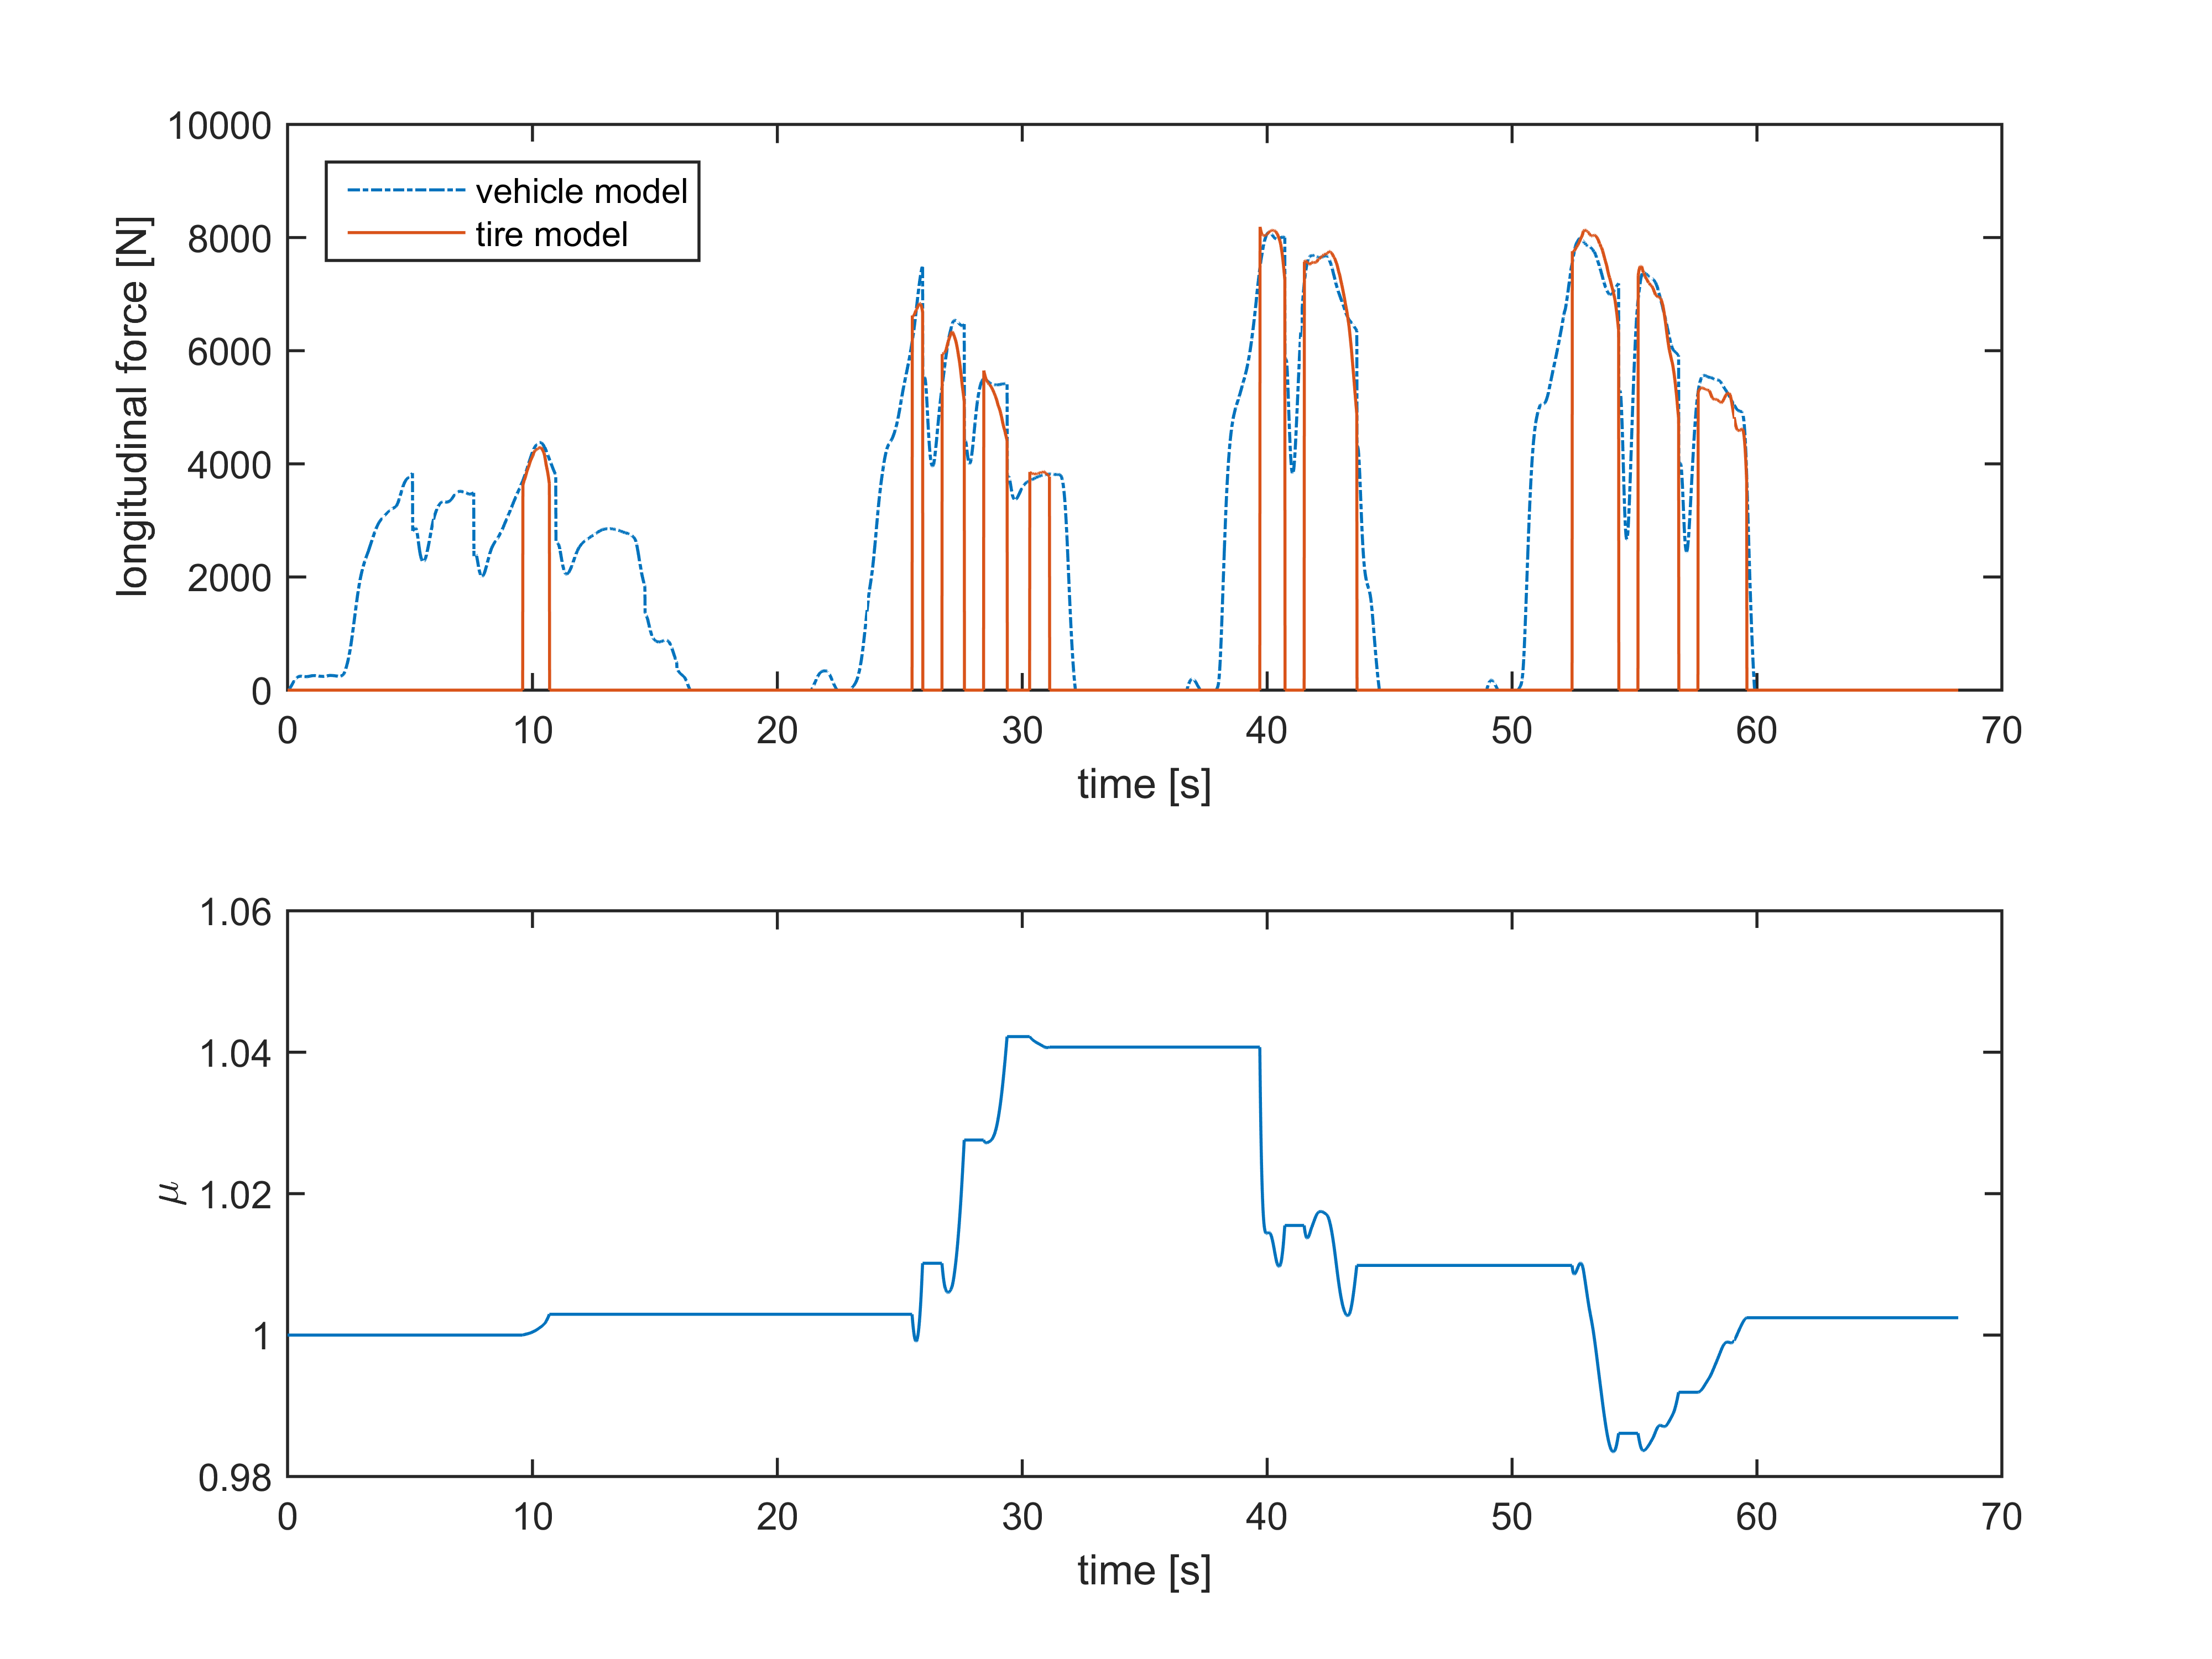
\includegraphics[width=1.0\textwidth]{Pictures/force_mue_olika_acc}
	\caption {Force from the tire and vehicle model and the approximated $ \mu $ for a straight line acceleration.}
	\label{force_mue_olika_acc}
\end{figure}

The friction estimation can seem to be jumpy at certain times, but the changes of frictional value are still quite small. The friction estimation stays around $ \mu = 1 $, which it evidently should due to the fact that the tire model parameters are fitted during this driving sequence. 

A more interesting test for the friction estimation algorithm is a driving sequence done as the fast track run. The same tires were used on a similar surface as in the previous driving sequence. The force from the two models and the friction estimation result can be see in Figure \ref{force_mue_race}. 

\begin{figure}[h]
	\centering
	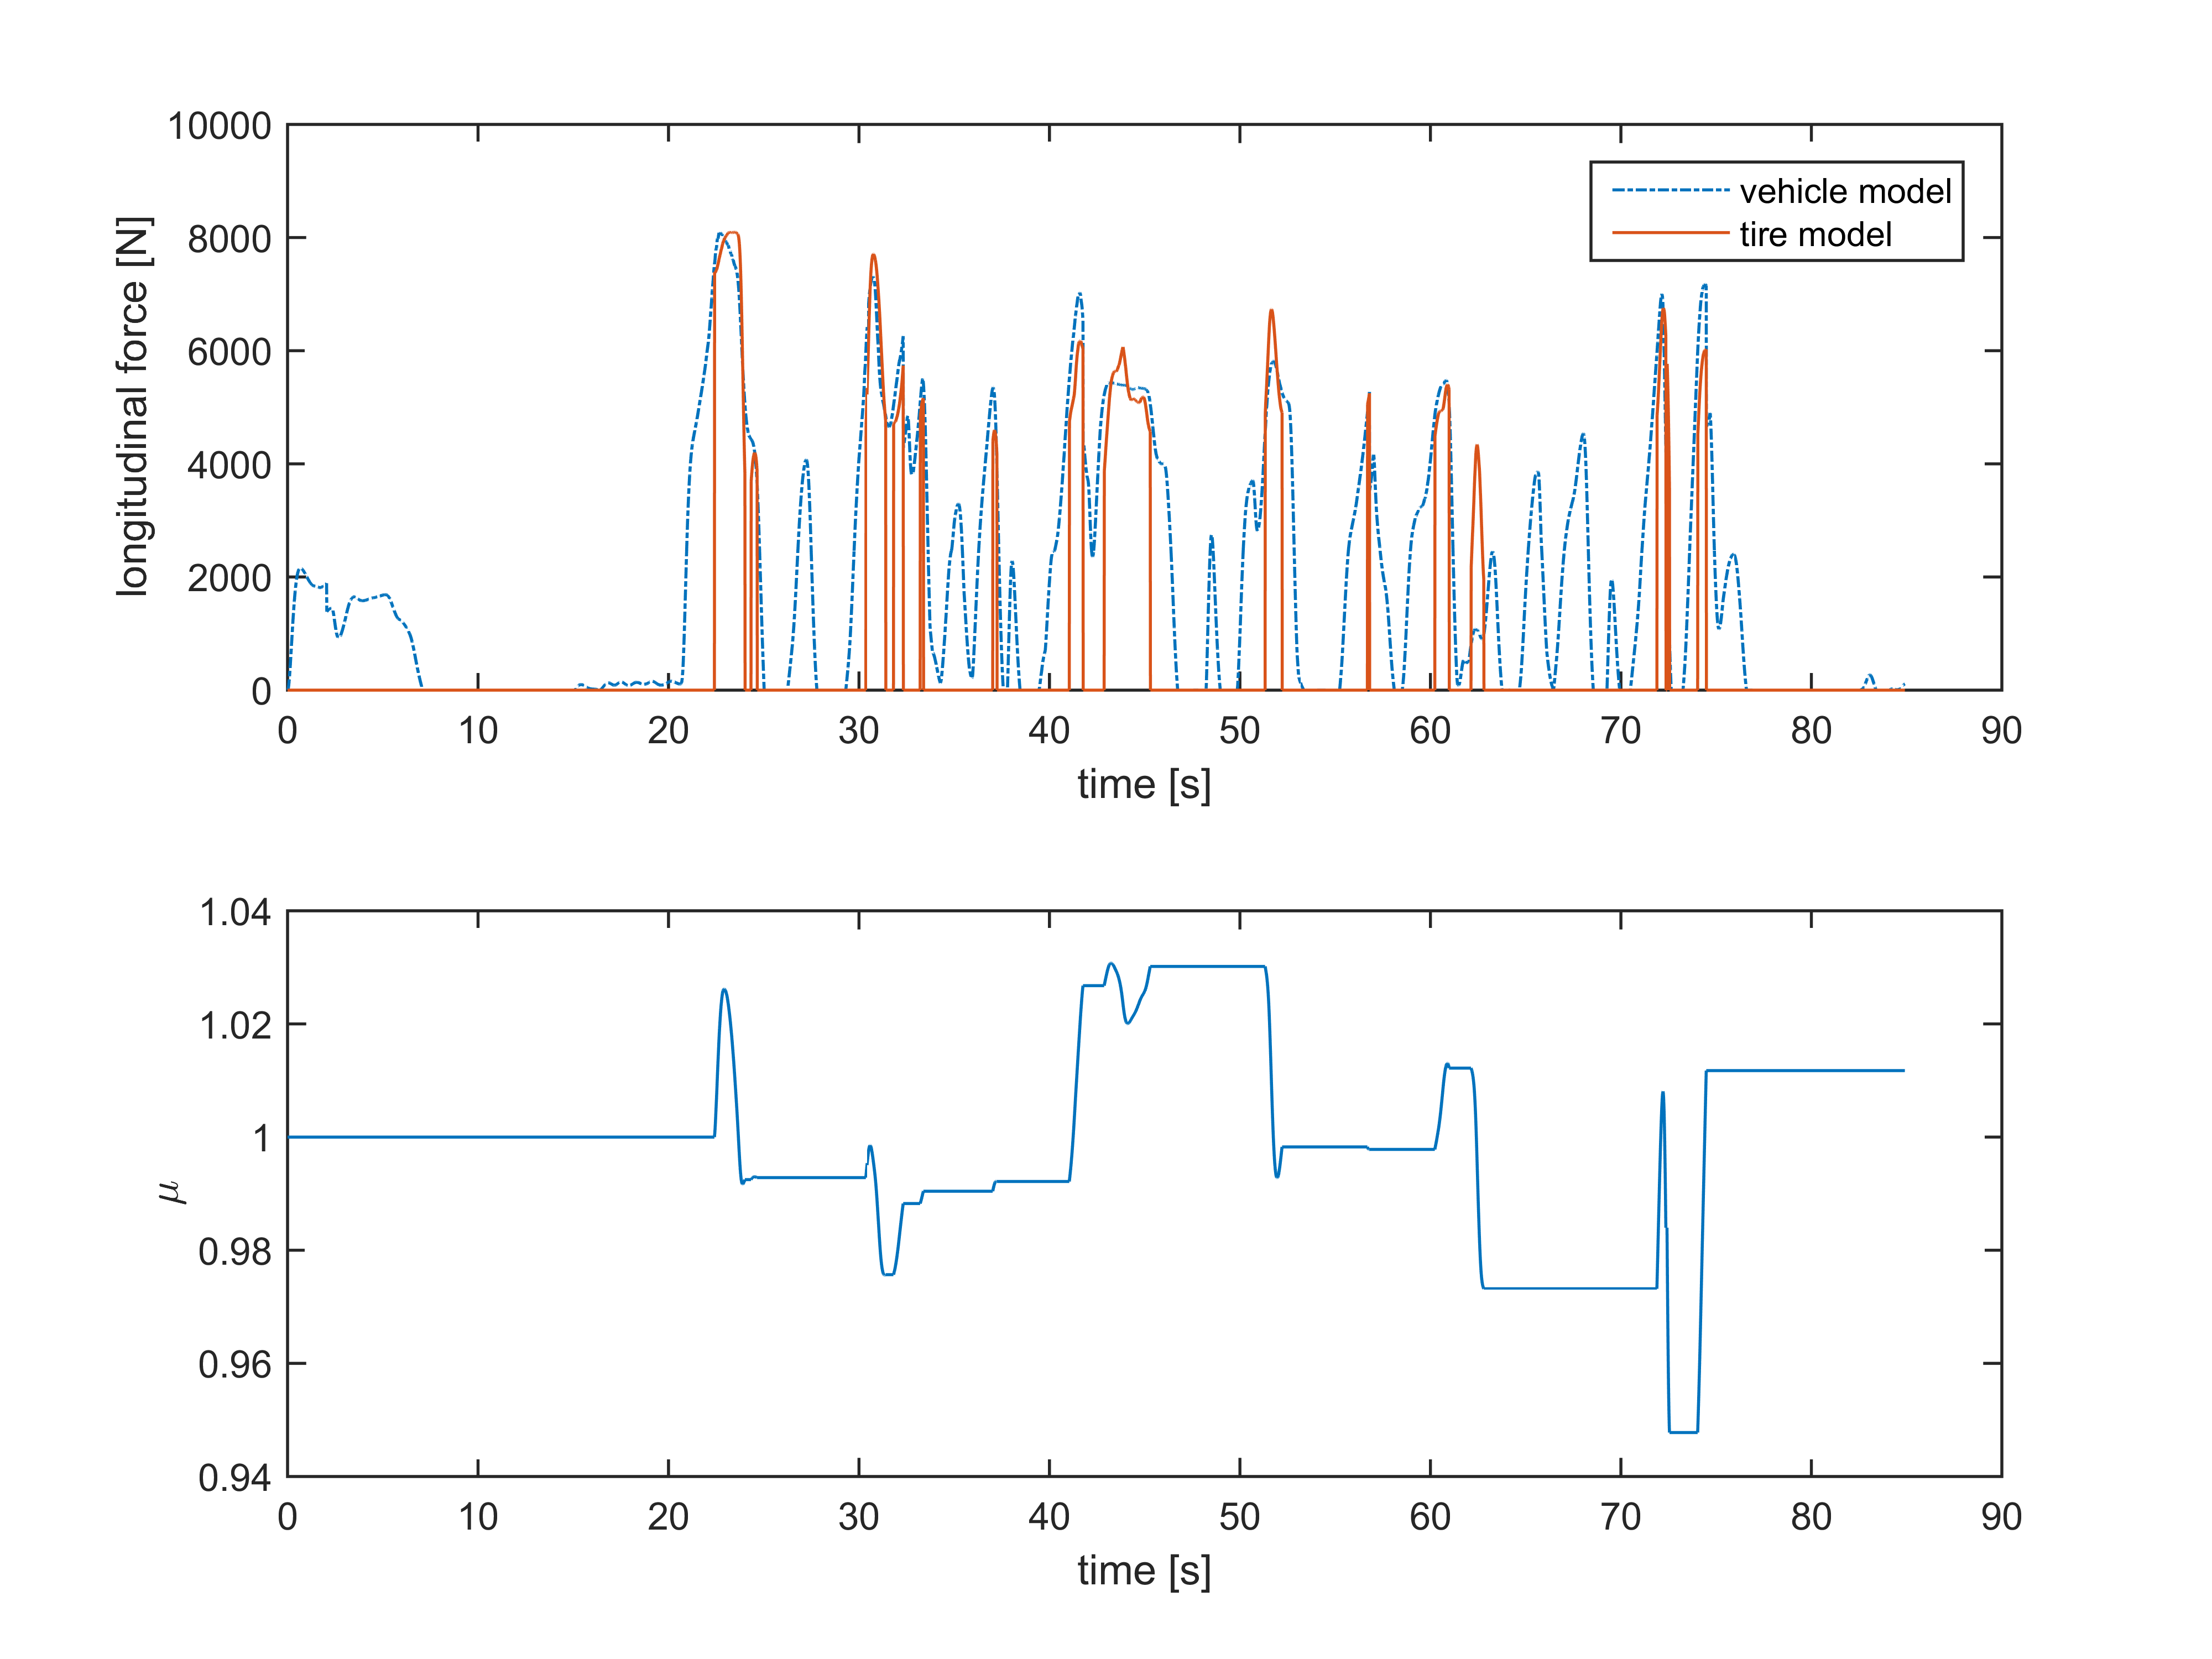
\includegraphics[width=1.0\textwidth]{Pictures/force_mue_race}
	\caption {Force from the tire and vehicle model and the approximated $ \mu $ for a fast track run.}
	\label{force_mue_race}
\end{figure}

The resulting friction coefficient is seen to vary around $ \mu = 1 $, similar to the straight line acceleration run. In the first subplot, it can be seen that the force from the tire model is calculated quite rarely, meaning that the friction coefficient is only approximated during these moment. However, the resulting $ \mu $ estimated during these moments are fairly steady around $ \mu = 1 $. 

\subsection{Winter tires on ice}
Being able to detect a surface with a low friction coefficient is probably the most important part of the friction estimation algorithm, due to the risk of an accident if too much torque is transferred to one of the driving axles. The resulting forces from the models and the approximated friction coefficient can be seen for a driving sequence on ice/snow in Figure \ref{force_mue_ice_normal}.

\begin{figure}[h]
	\centering
	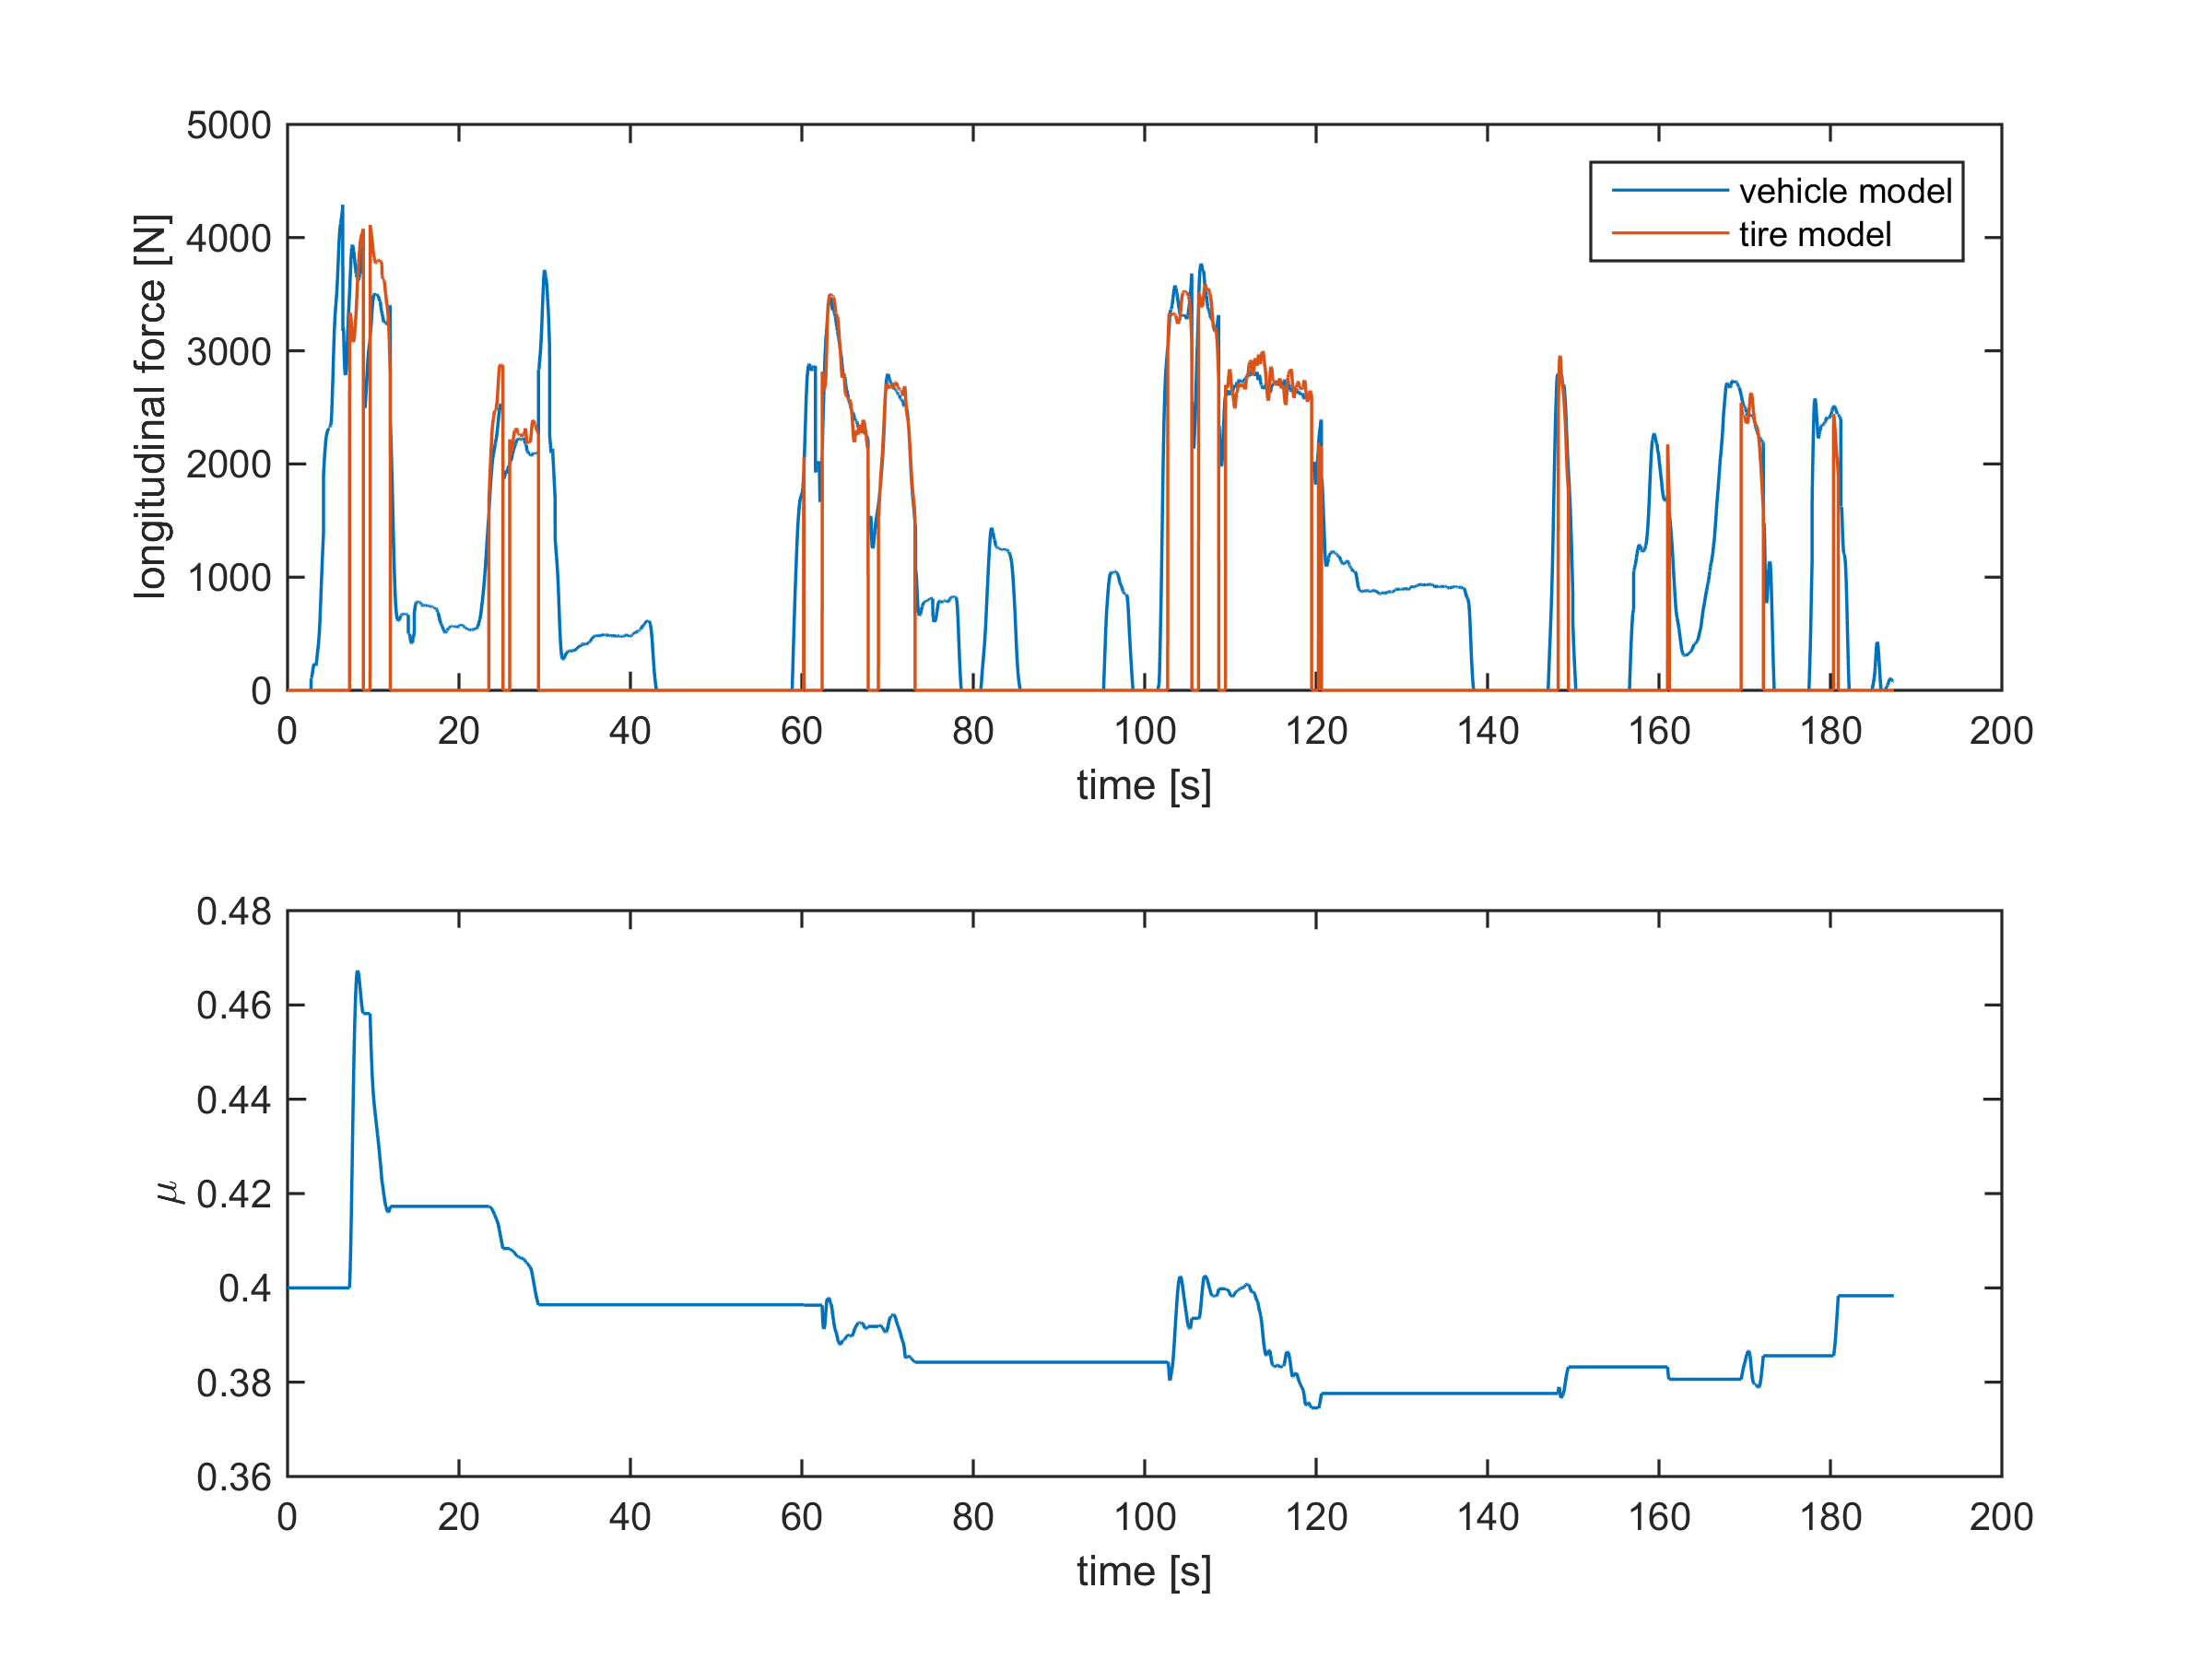
\includegraphics[width=1.0\textwidth]{Pictures/force_mue_ice_normal}
	\caption {Force from the tire and vehicle model and the approximated $ \mu $ for a driving sequence on ice/snow.}
	\label{force_mue_ice_normal}
\end{figure}

The winter tire model parameter for low-$ \mu $ was fitted on this run. It is therefore no coincidence that the friction coefficient end up at around $ \mu = 0.4 $. It can be seen in the figure that the force calculated from the tire model varies with a higher frequency during the driving sequence on ice/snow compared to the previous sequences. Even though, the resulting friction coefficient is approximated fairly well around friction $ \mu = 0.4 $, especially when the approximation algorithm is active for a relatively large period of time seen at $ \approx 100-120 $ s. A quite large disturbance of $ \mu $ can unfortunately be seen at the times $ \approx 7 - 12$ s.

\subsection{Winter tires on asphalt and ice combined}
The main goal for the work done in this report was to detect when low-$ \mu $ is present so that the torque transfer through the FXD can be limited. It is therefore essential to test the developed algorithm during a driving sequence that actually includes a change of $ \mu $, preferably from high-$ \mu $ to low-$ \mu $, to verify that the algorithm can handle this kind of abrupt change. It has not been possible to test this on a single run, for example using a driving sequence that includes both asphalt as well as a skid pad. In order to simulate this behavior, two different runs have been merged together, where the friction coefficient changes a total of three times. Starting at high-$ \mu $ and finishing with low-$ \mu $. The merging was made at points where both sequences were accelerating or decelerates at the same velocity, in order to avoid unnecessary jumps of other signals from the vehicle. 

The two modeled forces and the resulting $ \mu $ from the merged run can be seen in Figure \ref{force_mue_comb2}. The approximated friction coefficient is seen to clearly change when a different driving sequences is begun, meaning that the algorithm manages to detect that the grip between the tire and the road differs.
 
\begin{figure}[h]
	\centering
	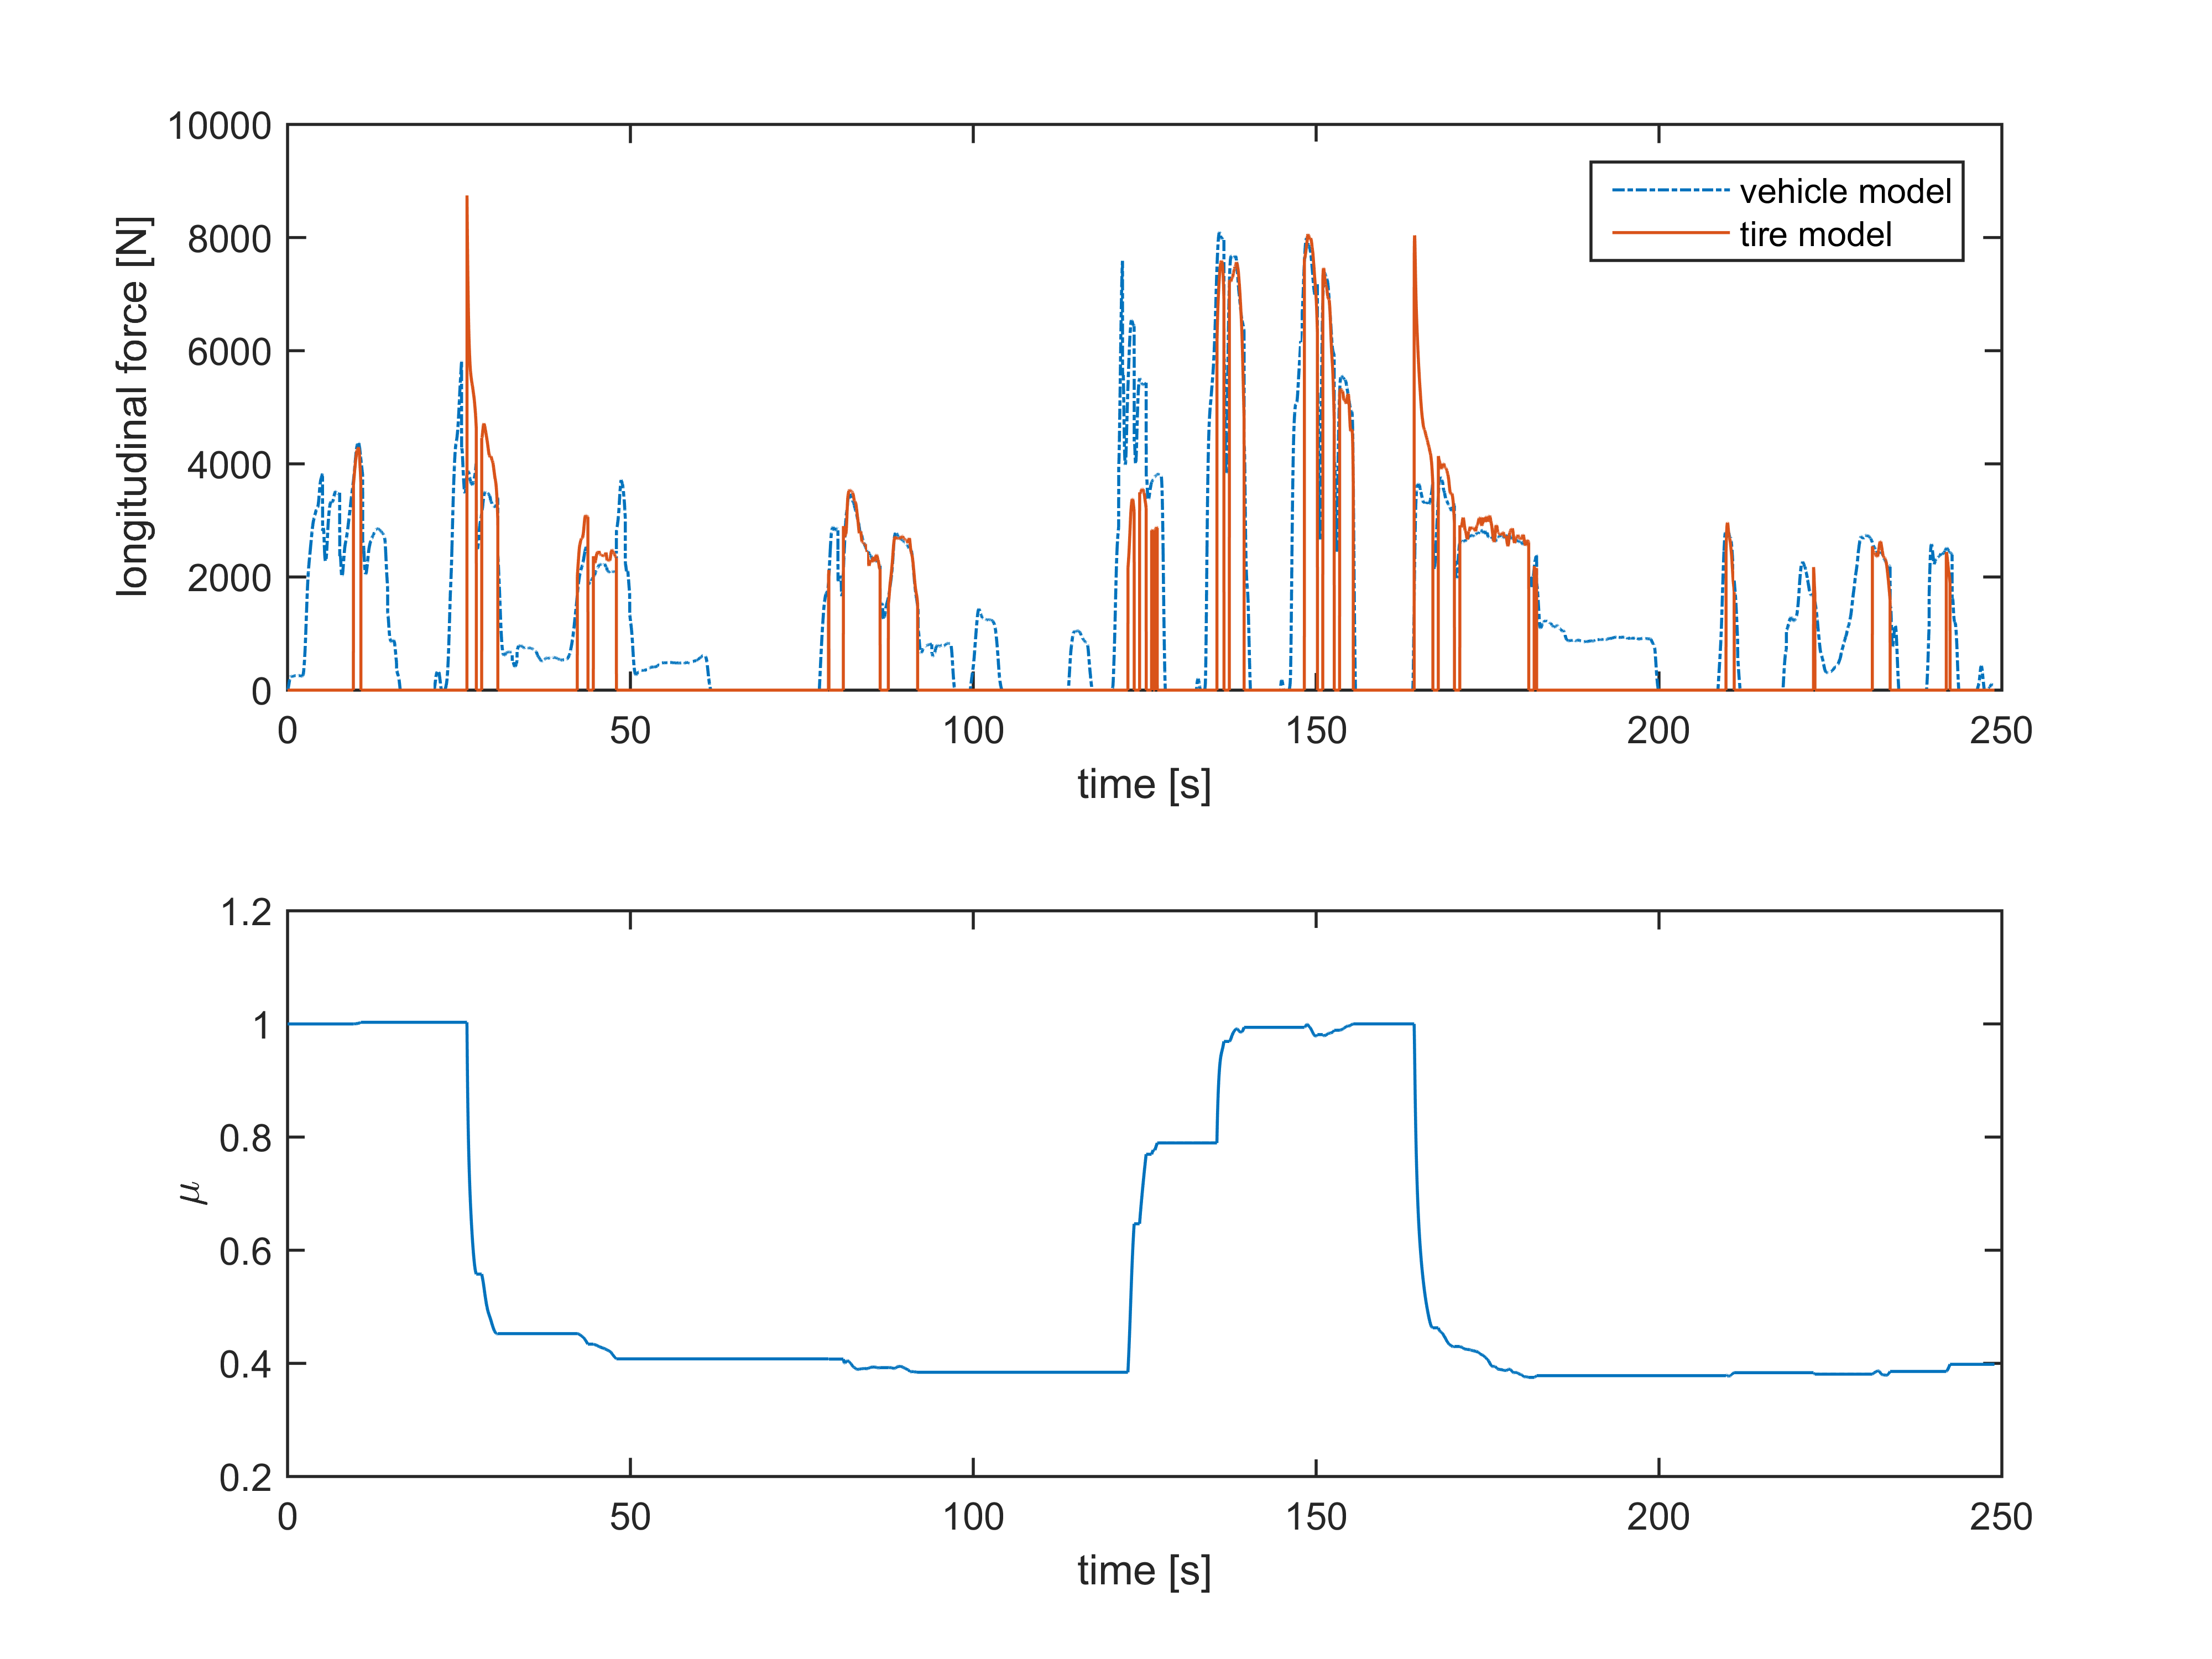
\includegraphics[width=1.0\textwidth]{Pictures/force_mue_comb2}
	\caption {Force from the tire and vehicle model and the approximated $ \mu $ for two different runs merged together.}
	\label{force_mue_comb2}
\end{figure}

Due to the limitations set concerning when the friction coefficient should be approximated (Section \ref{when_to_estimate}), the algorithm may not update $ \mu $ at the same instance as the new surface is present. However, when the algorithm is allowed to approximate, the new friction coefficient is approximated with good speed. In Figure \ref{force_mue_comb2_zoom}, the two forces and the friction coefficient can be seen when the result is zoomed in on a sudden drop of the friction coefficient. The converging $ \mu $ is seen to drop very fast as the two forces differs greatly right after $ \approx 26.2 $ s, and thereafter decrease more slowly. 

\begin{figure}[h]
	\centering
	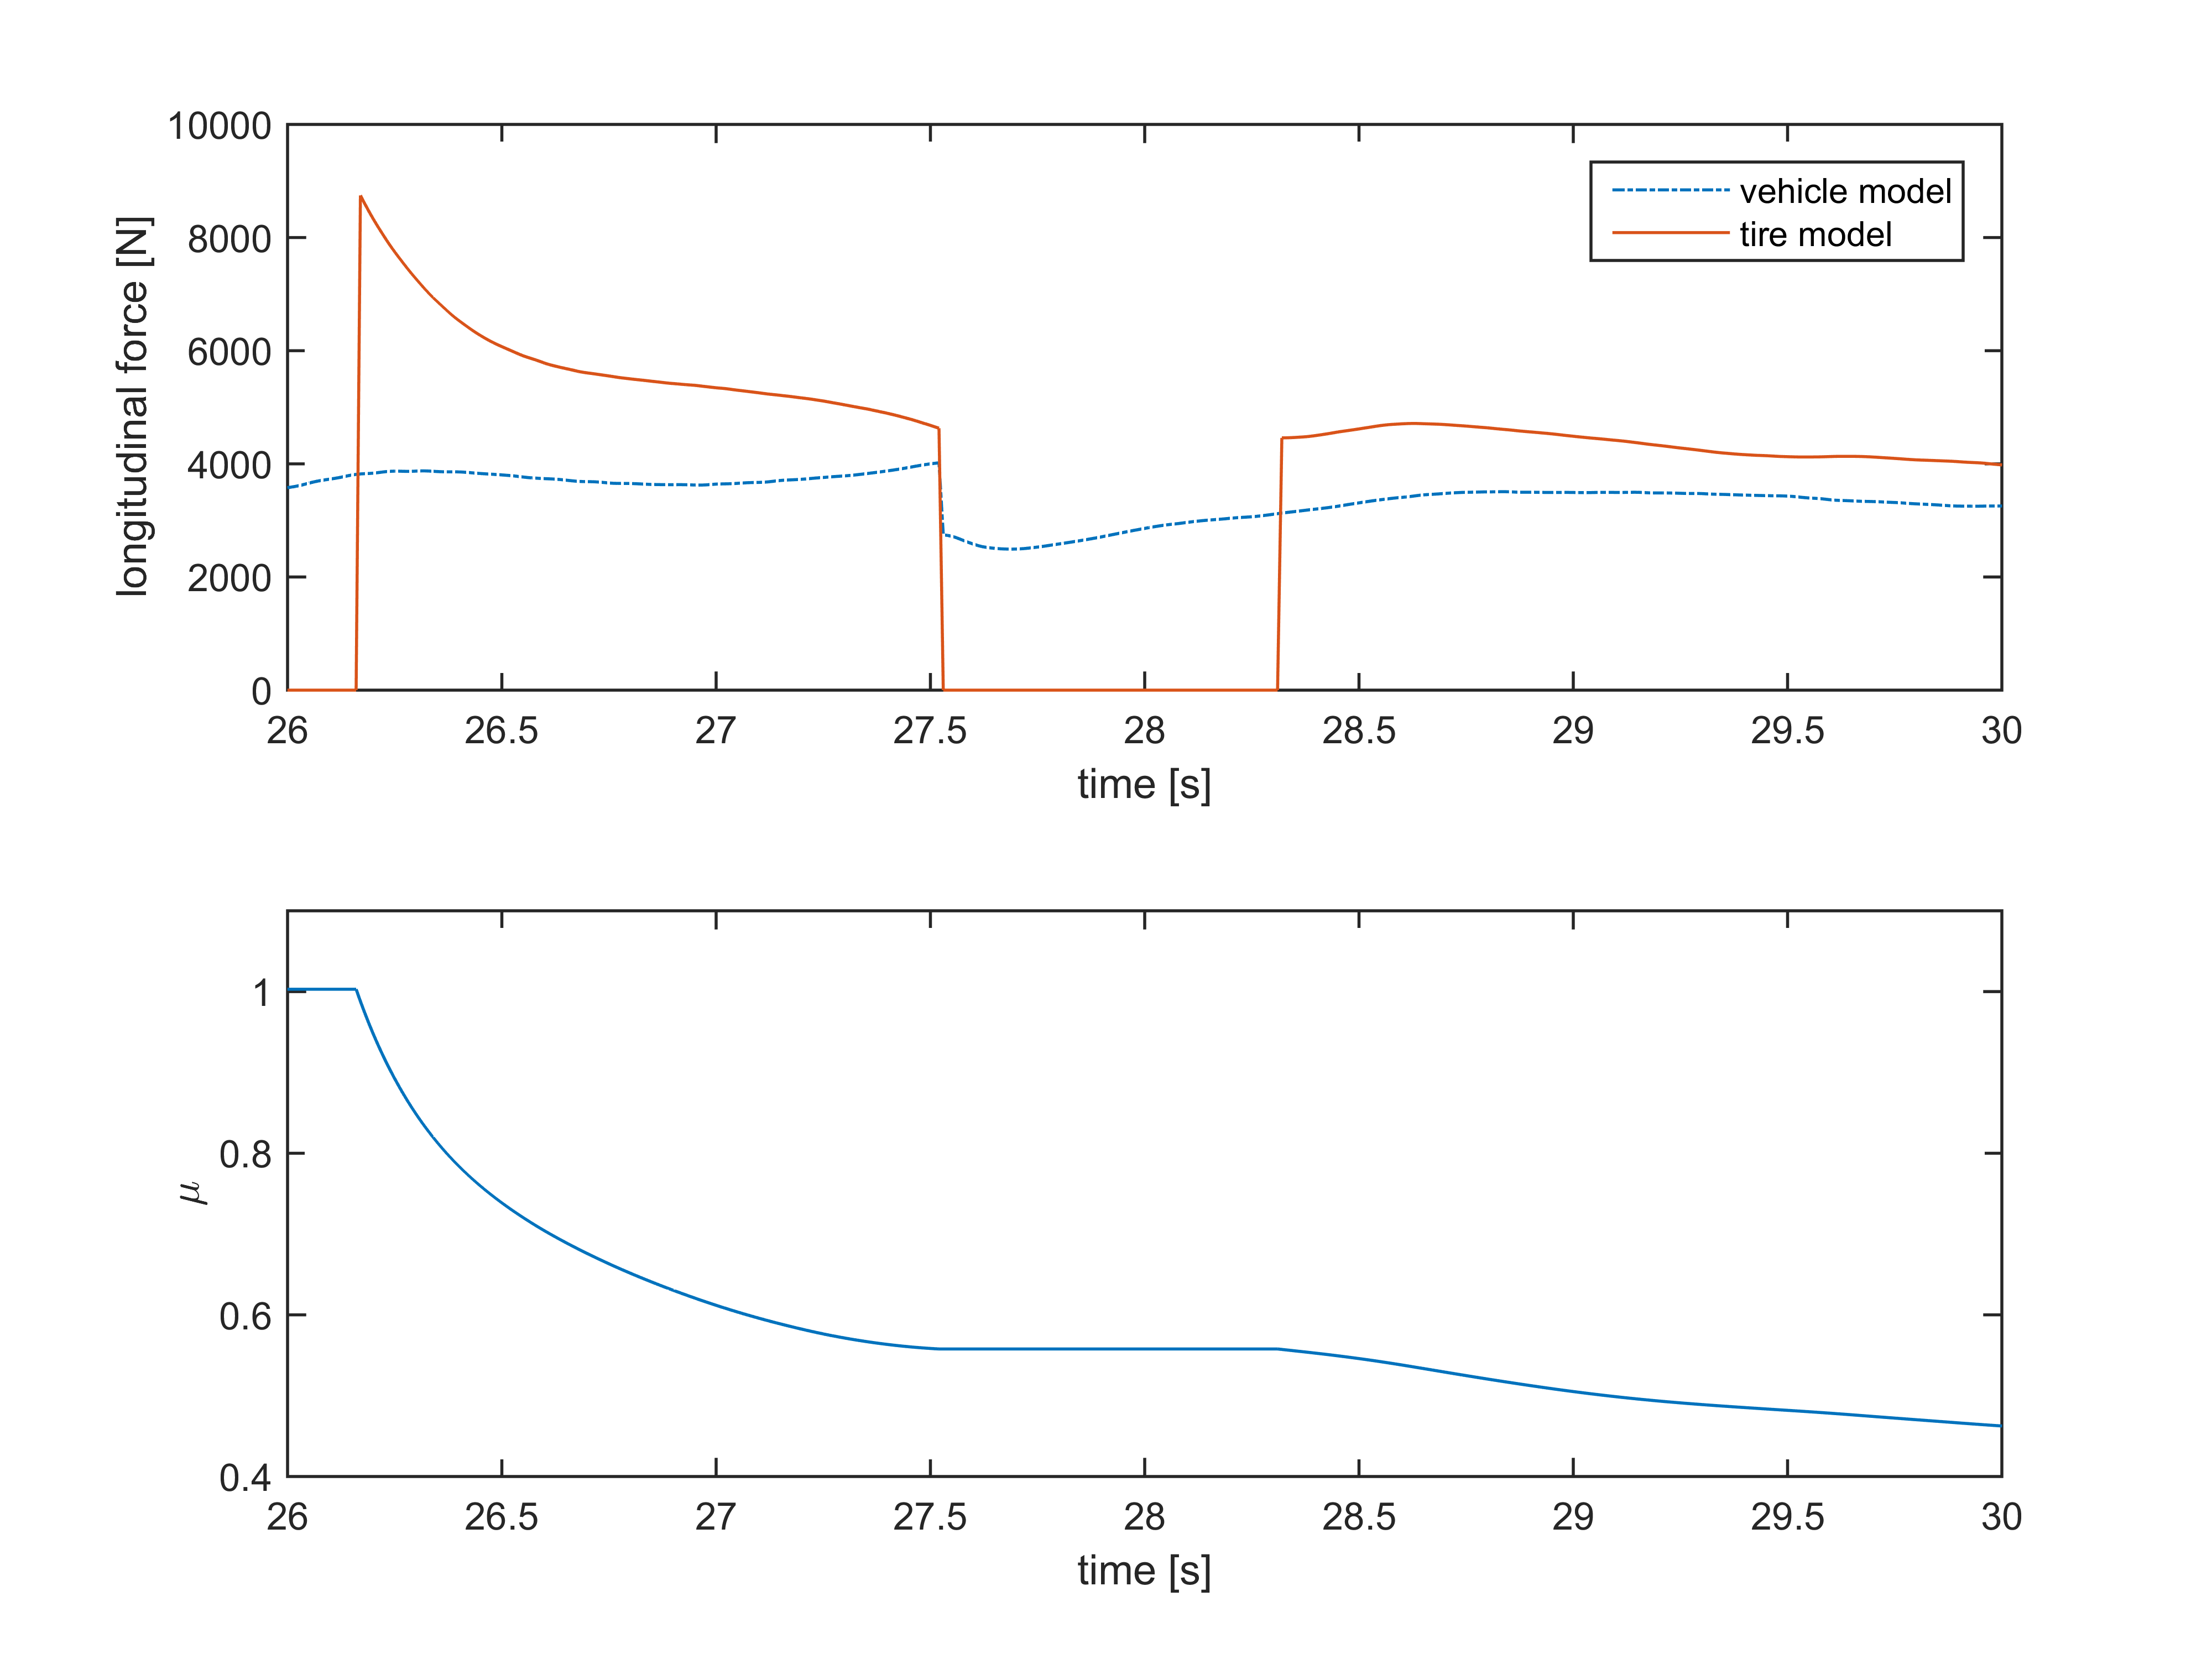
\includegraphics[width=1.0\textwidth]{Pictures/force_mue_comb2_zoom}
	\caption {Zoomed in picture of Figure \ref{force_mue_comb2}, showing how fast the new friction coefficient is found.}
	\label{force_mue_comb2_zoom}
\end{figure}

The normalized force per slip ratio curve for the combined sequence can be seen in Figure \ref{slip_kraft_comb2}. Note that this figure is merely the two Figures \ref{slip_kraft_ljungby} and \ref{slip_kraft_is} added on top of each other, with some erroneous result due to the wrong calculated force when the friction coefficient suddenly changes. The result clearly shows that a tire's stiffness varies for surfaces.

\begin{figure}[h]
	\centering
	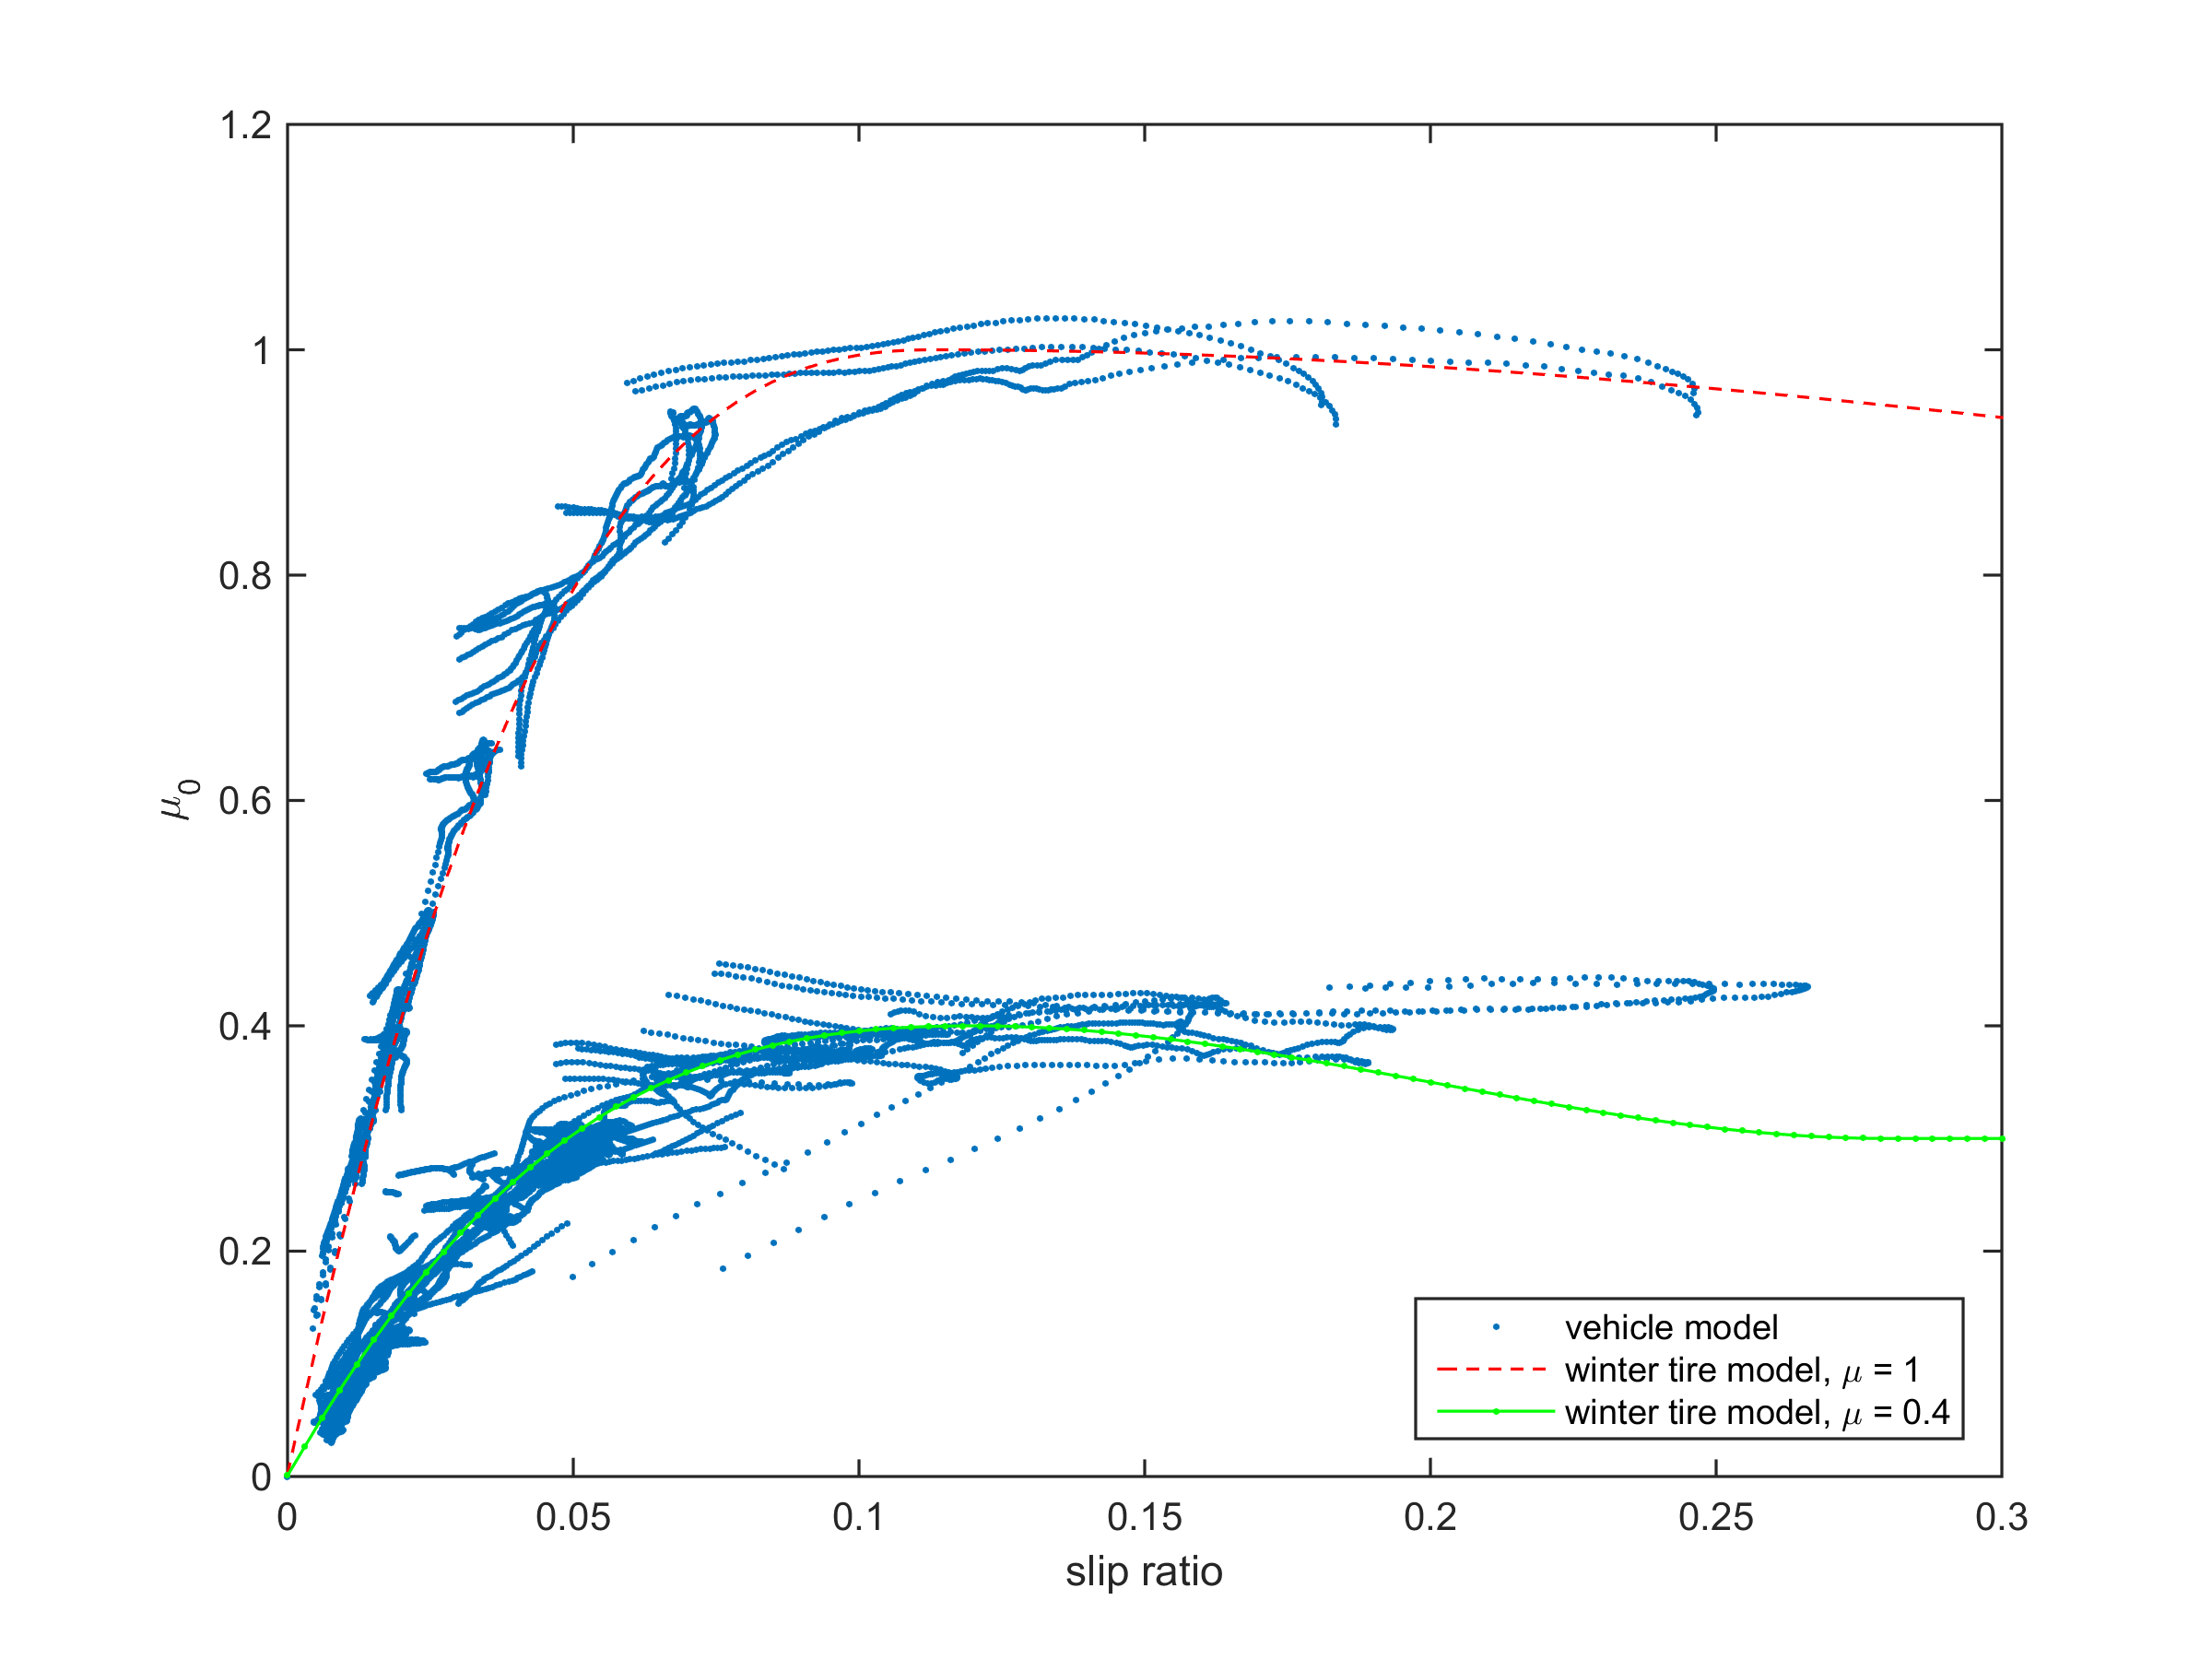
\includegraphics[width=1.0\textwidth]{Pictures/slip_kraft_comb2}
	\caption {Force per slip ratio for the combined driving sequence with both low- and high-$ \mu $.}
	\label{slip_kraft_comb2}
\end{figure}

\subsection{Summer tires on asphalt}
A fast track lap was also run with the summer tires on asphalt. These tires were, as mentioned before, relatively stiff and with the peak force located at a relative small slip ratio value. This resulted in a tougher tire force modeling where smaller variances gave larger errors. 

The result from this fast track run can be seen in Figure \ref{force_mue_race_bb}. The two first curves, \textit{vehicle model} and \textit{tire model, used value}, are the same calculations as seen earlier in the result, where \textit{tire model, used value} are only calculated when the conditions are met in Section \ref{when_to_estimate}. These conditions are not met at any longer times, as the figure shows, even though the forces acting are relatively high at numerous times. Therefore the curve \textit{tire model, all value} is shown to demonstrate why the conditions for the friction estimation algorithm are not met.

\begin{figure}[h]
	\centering
	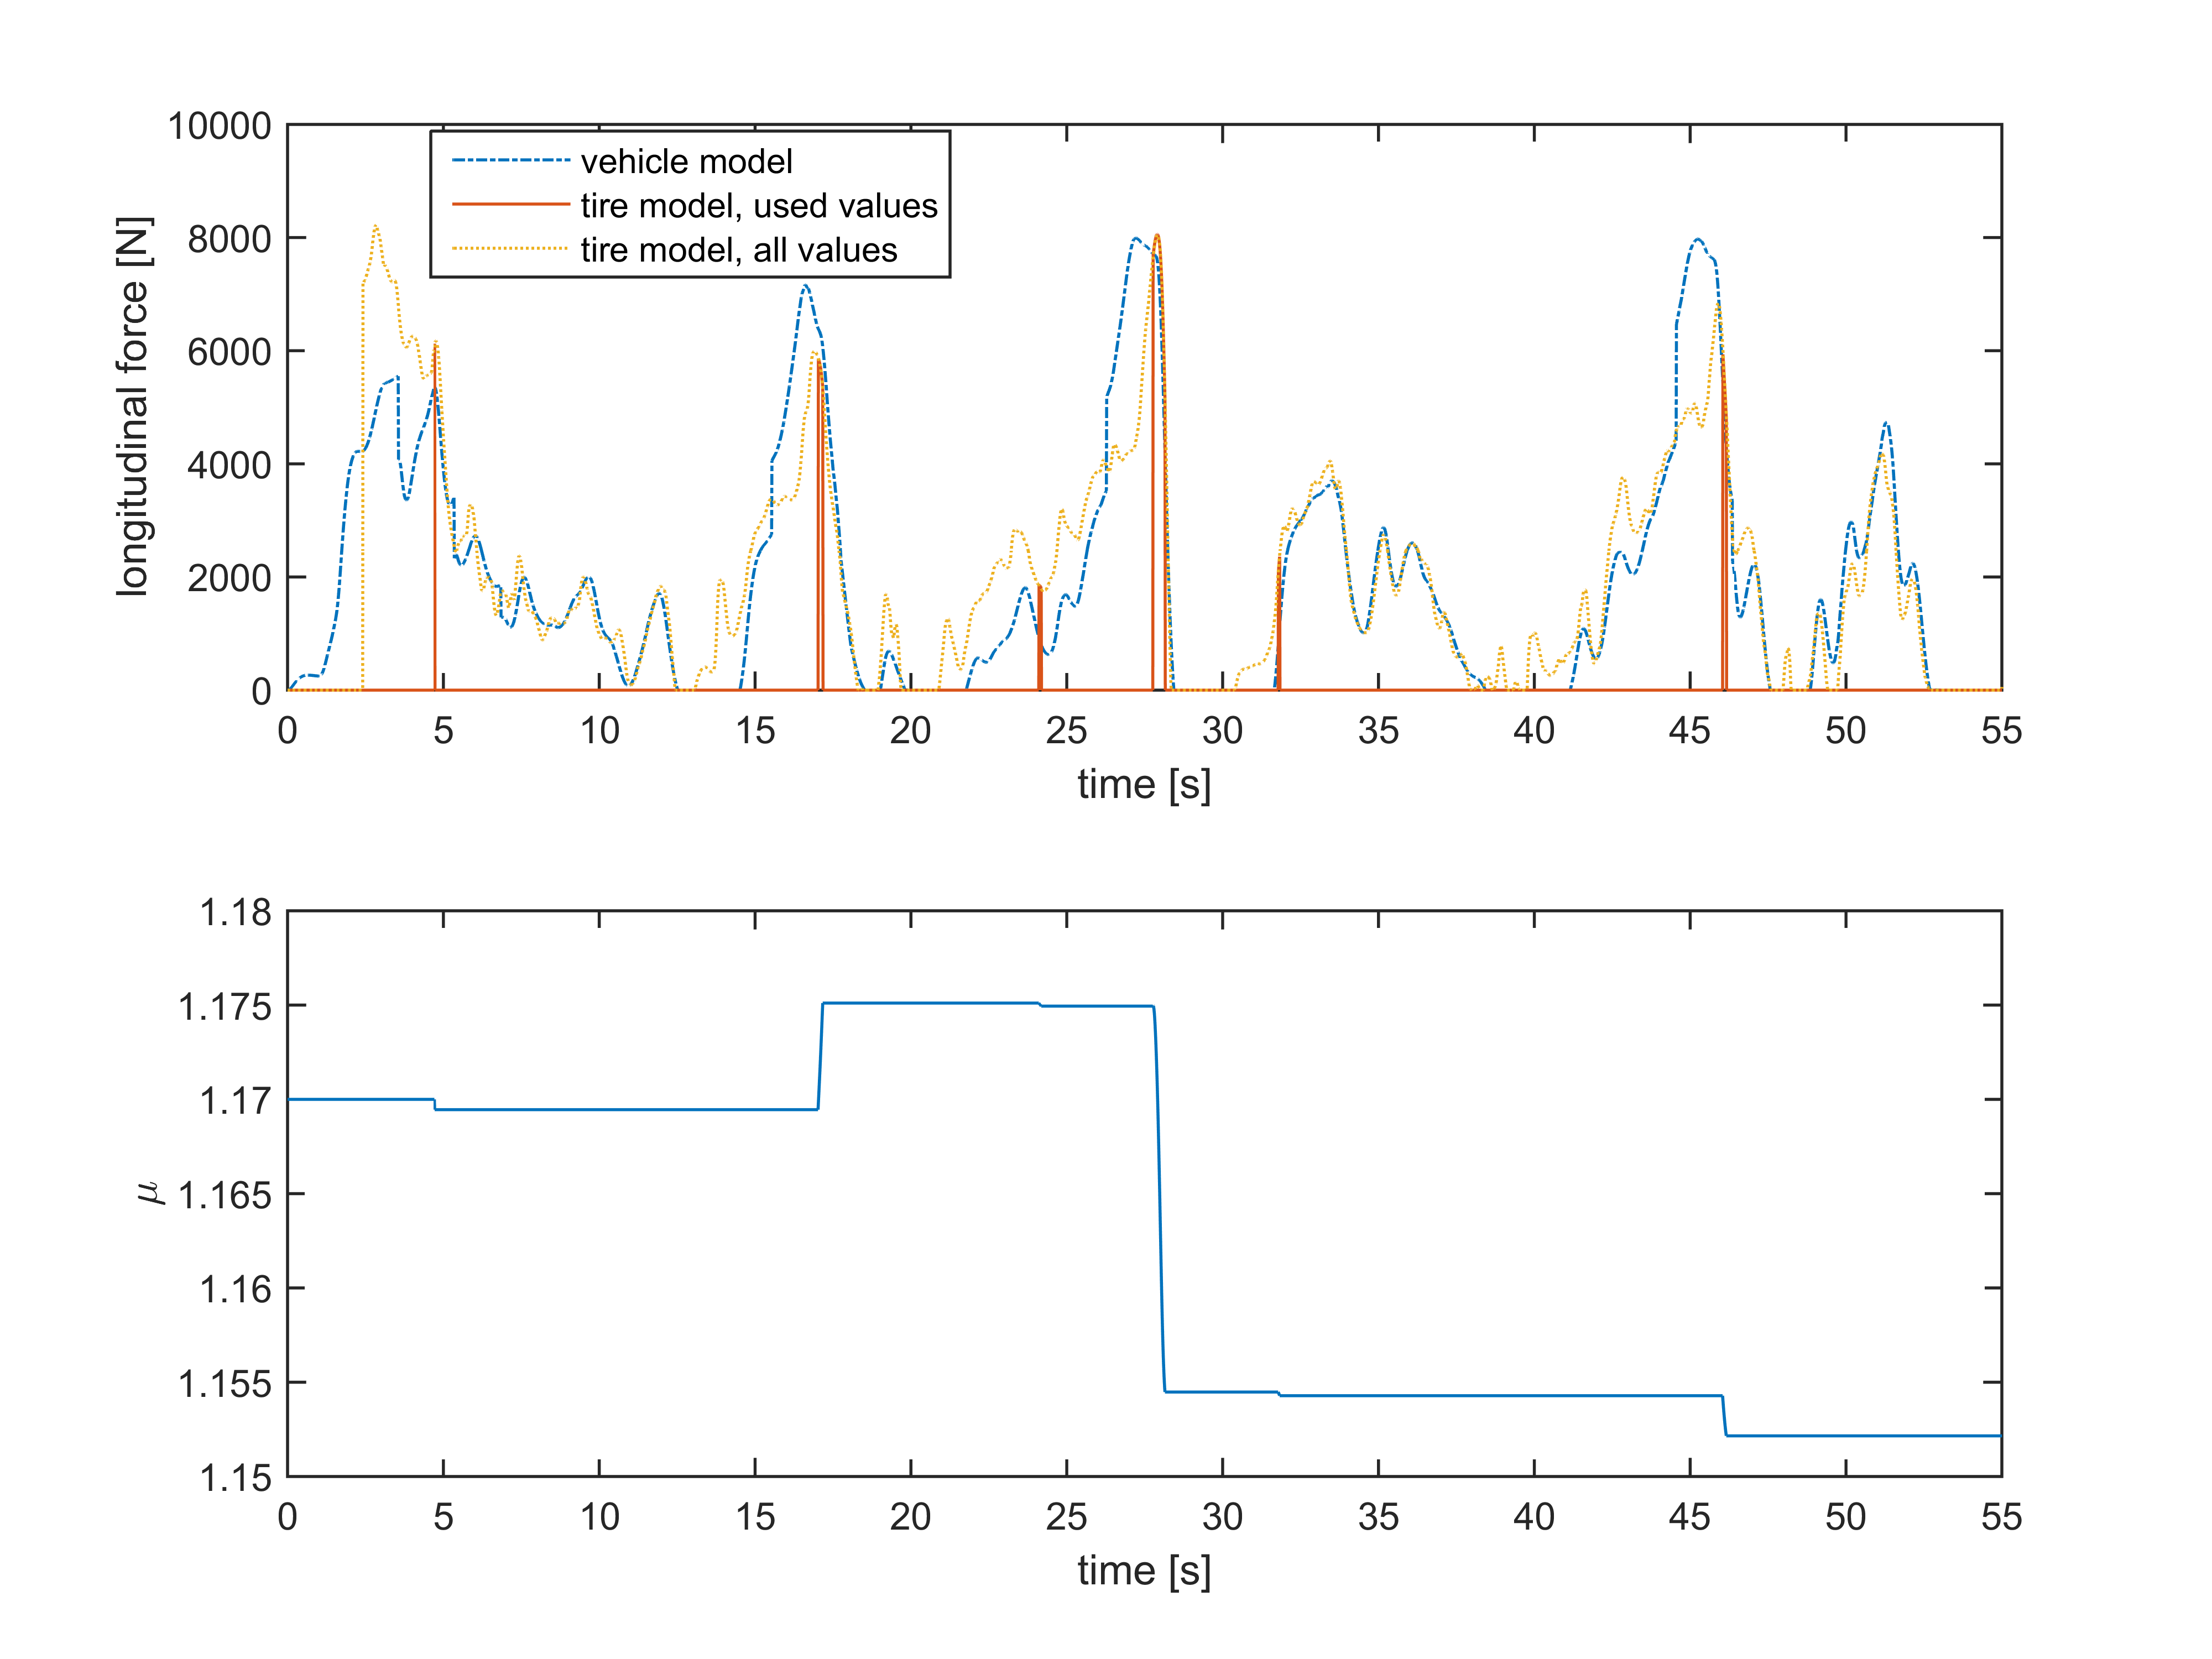
\includegraphics[width=1.0\textwidth]{Pictures/force_mue_race_bb}
	\caption {Force from the tire and vehicle model and the approximated $ \mu $ for a driving sequence on asphalt with summer tires.}
	\label{force_mue_race_bb}
\end{figure}

\subsection{Summer tires on wet asphalt}
A similar fast track lap was done with the summer tires on wet asphalt, to test the algorithm's behavior on the same road surface but with different driving conditions. The result from this driving sequence can be seen in Figure \ref{force_mue_race_bb}. It can be seen that the resulting $ \mu $ does not drop much lower than the $ \mu = 1.17 $ that calculated on the dry acceleration run. 

\begin{figure}[h]
	\centering
	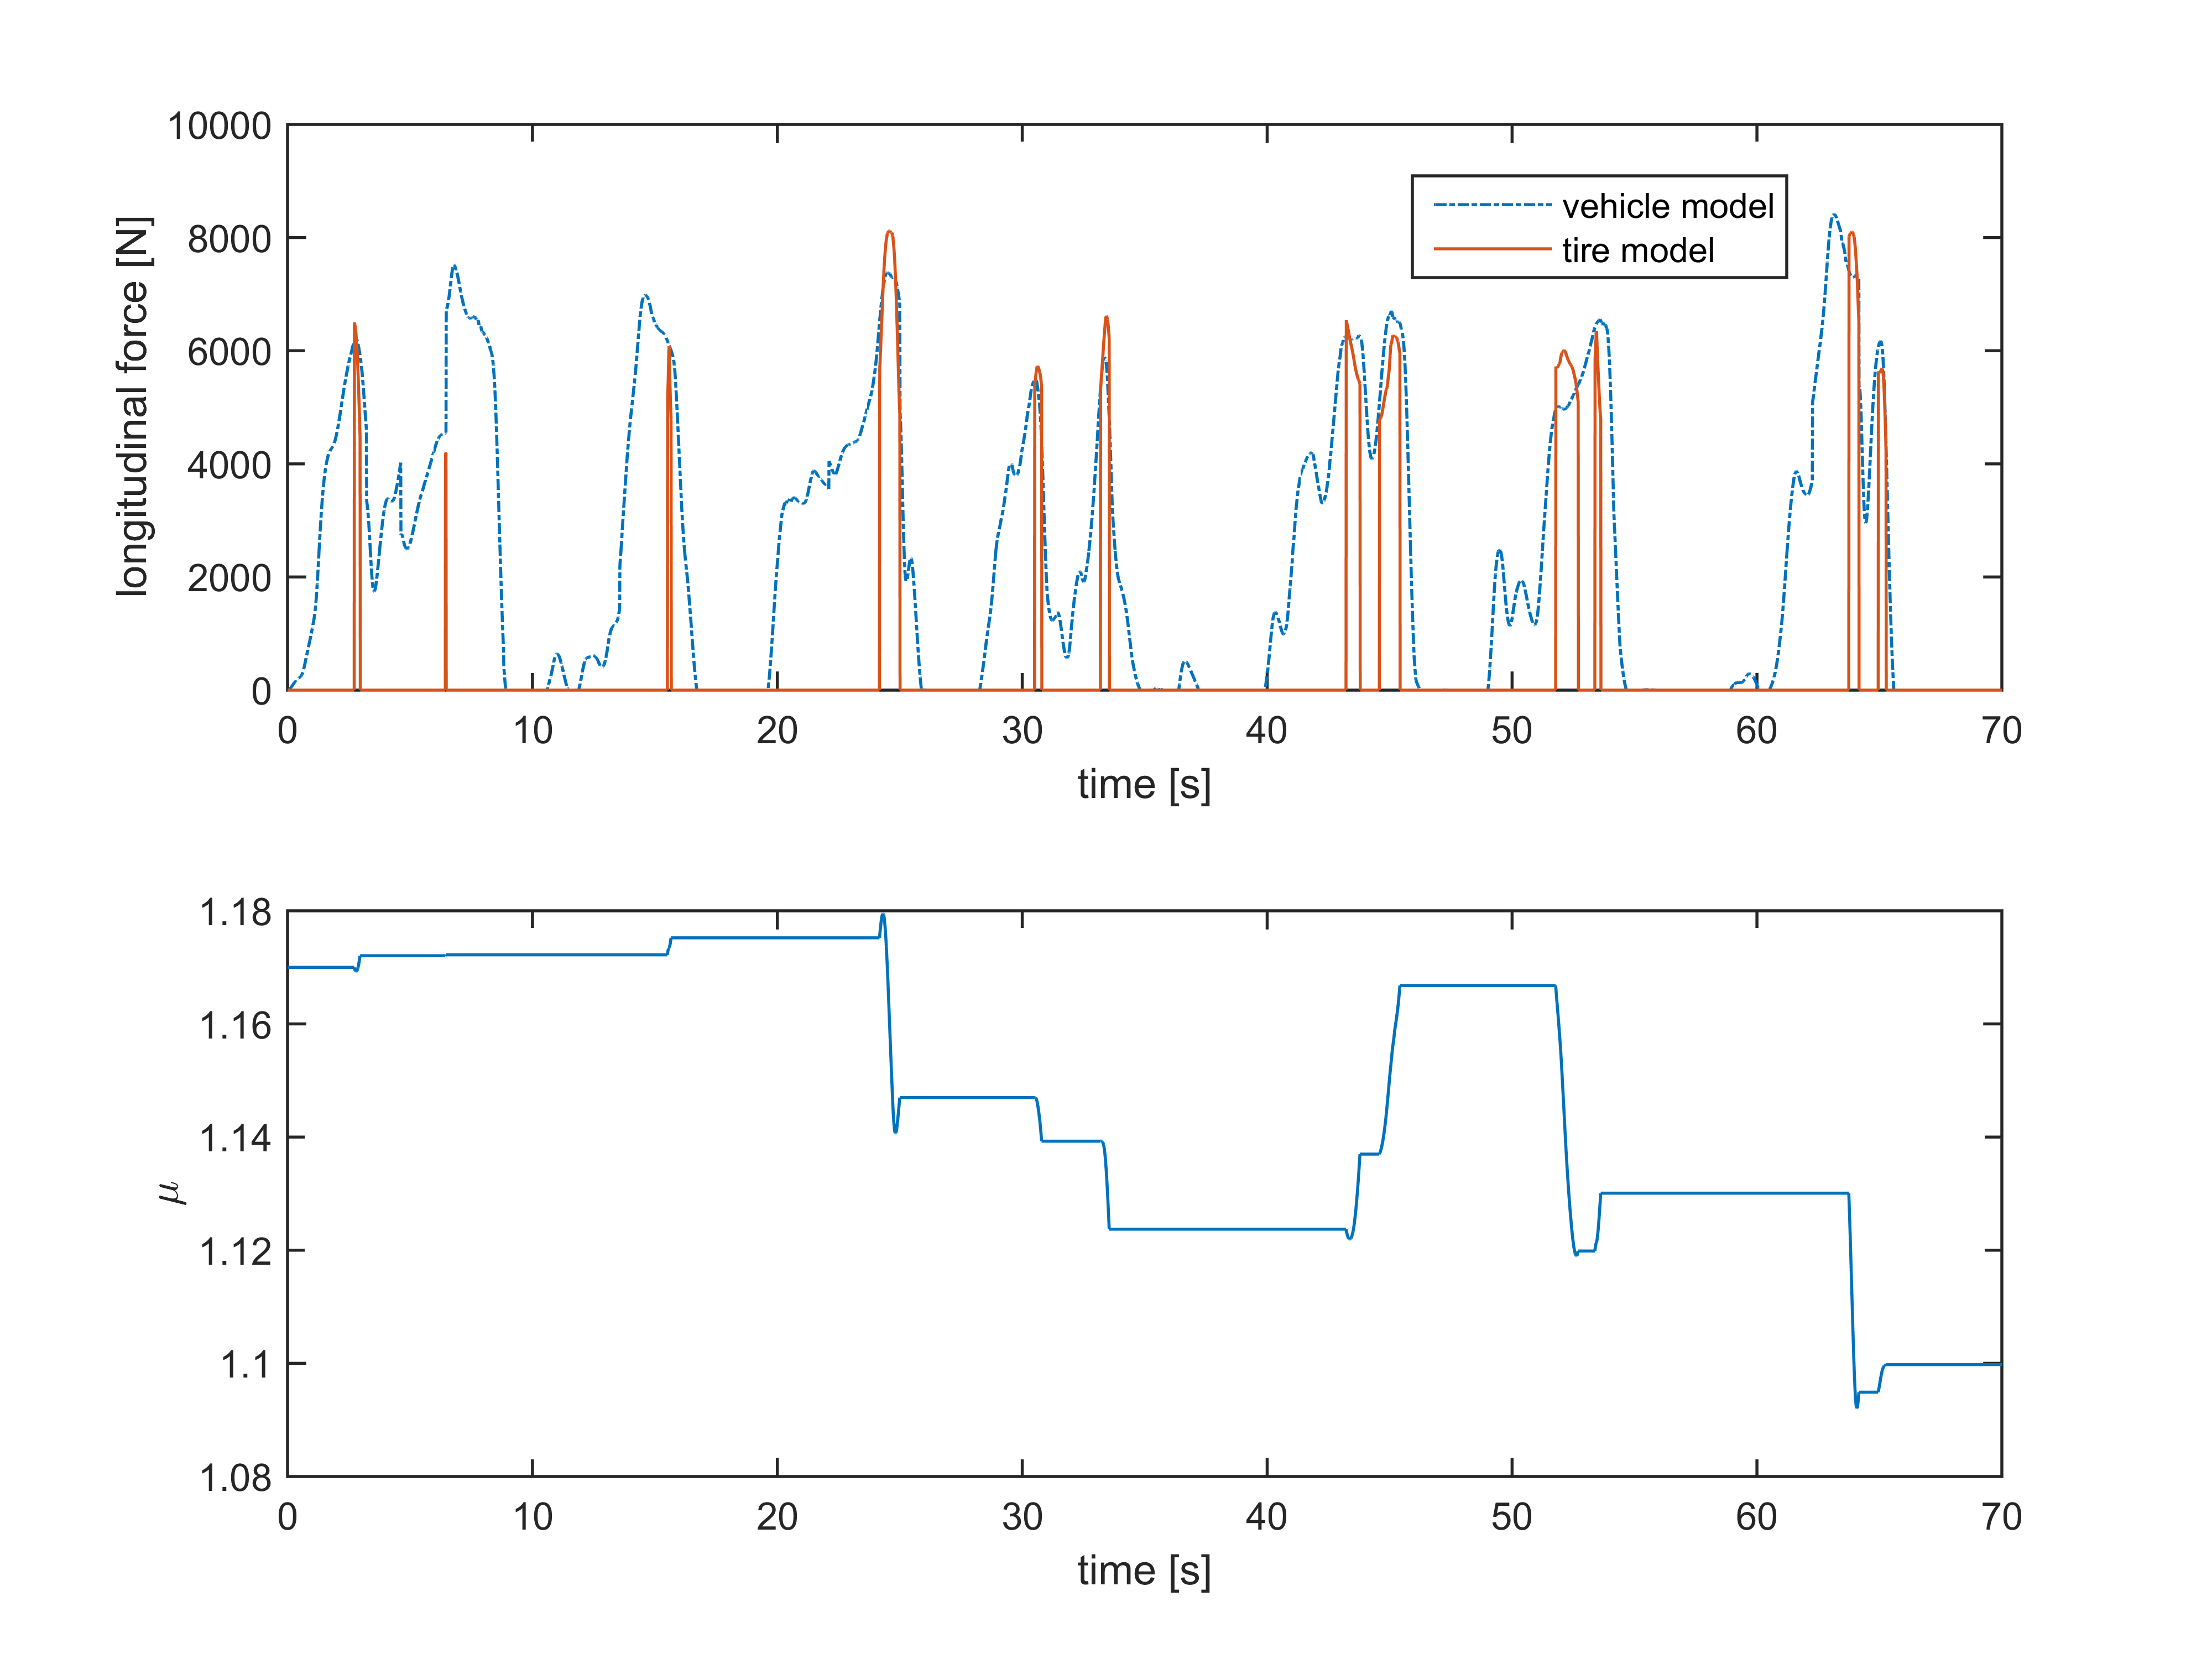
\includegraphics[width=1.0\textwidth]{Pictures/force_mue_blot_race_bb}
	\caption {Force from the tire and vehicle model and the approximated $ \mu $ for a driving sequence on asphalt with summer tires.}
	\label{force_mue_blot_race_bb}
\end{figure}

In Figure \ref{slip_kraft_blot_och_torr} the normalized force for the two similar acceleration runs can be seen. The first subplot corresponds to dry asphalt and the second subplot corresponds to wet asphalt, where the dashed line in the two plots are described by exactly the same tire model parameters. The figure shows that the longitudinal force per slip ratio is not decreased when accelerating on wet asphalt. 

\begin{figure}[h]
	\centering
	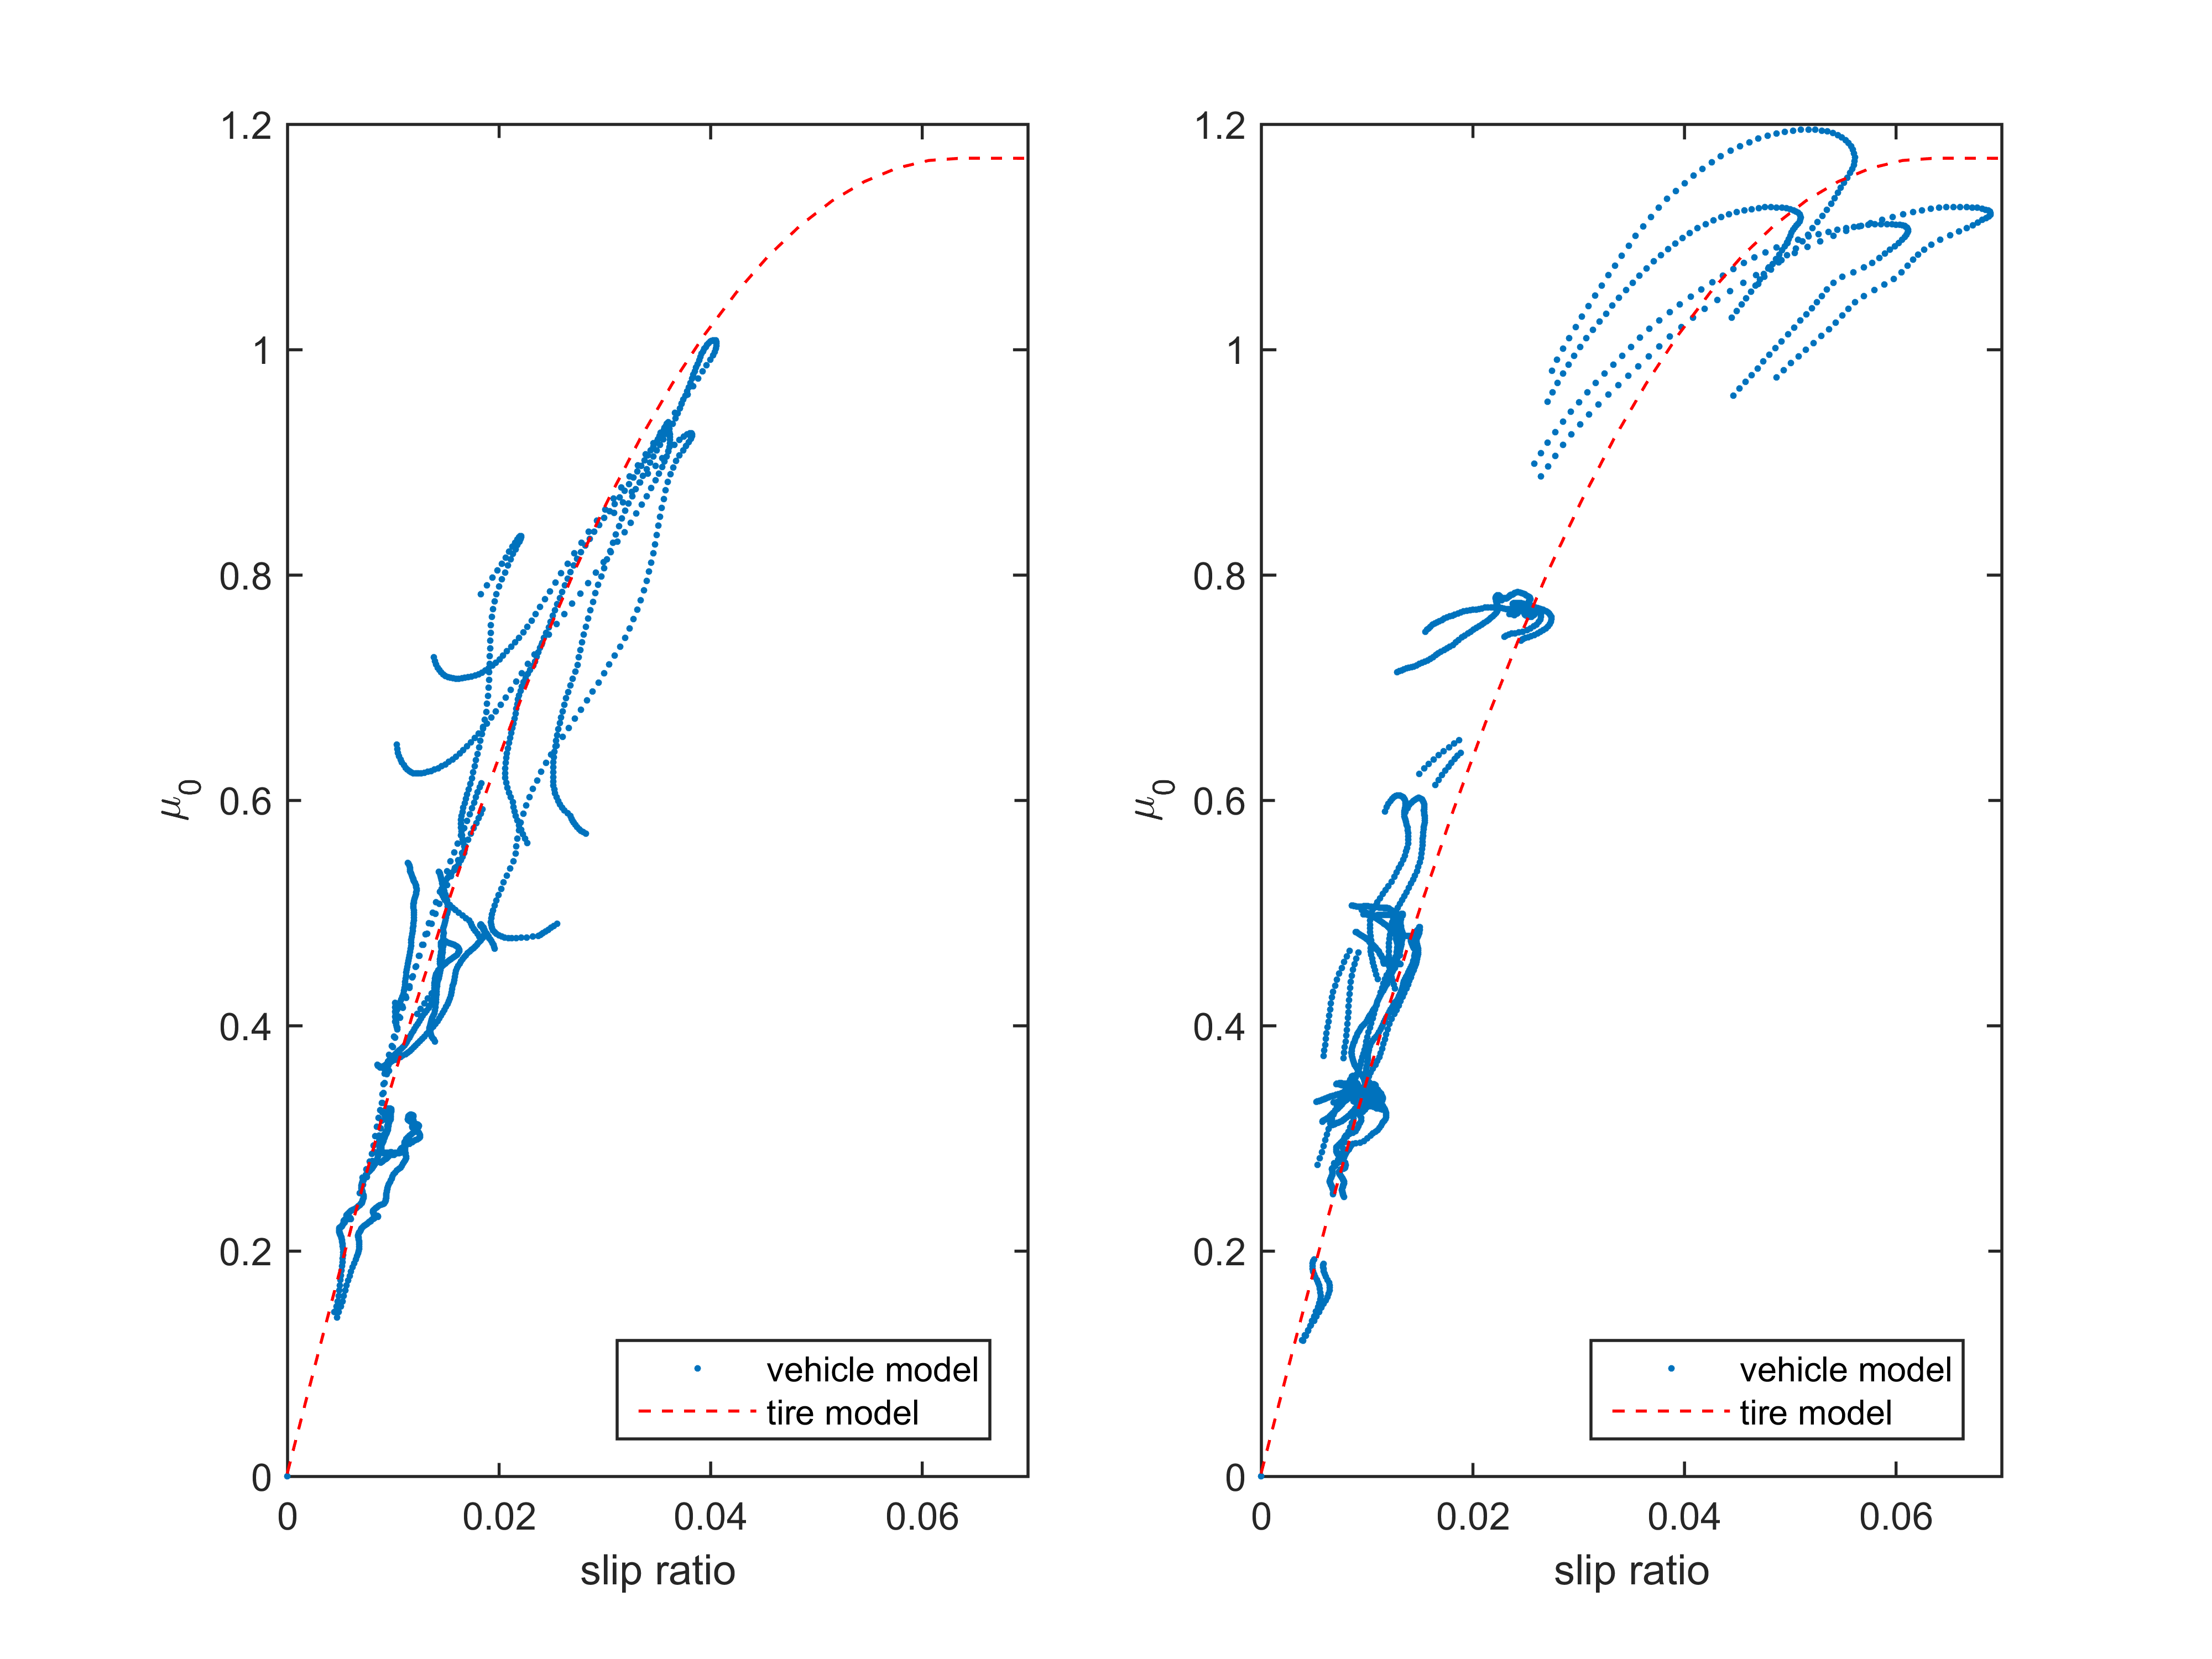
\includegraphics[width=1.0\textwidth]{Pictures/slip_kraft_blot_och_torr}
	\caption {Normalized force per slip ratio. Subplot one for dry asphalt and subplot two for wet asphalt.}
	\label{slip_kraft_blot_och_torr}
\end{figure}
